\documentclass[praxisarbeit,english,oneside]{framework/hgbthesis}
\graphicspath{{images/}}            % wo liegen die Bilder? 
\bibliography{default/literatur}  	% Angabe der BibTeX-Datei

\makenoidxglossaries                % Glossarbefehl
\loadglsentries{default/glossary}   % Laden der Glossareinträge aus der Datei

%%%----------------------------------------------------------
\begin{document}
%%%----------------------------------------------------------
\visibleTodos{true} % Sollen TODOs angezeigt werden ? (true/false)

% Einträge für Titelblatt: --------------------------------
\title{Designing a Network-based Cinema Management Solution using Code Generation}
\pruefer{Prof. Dr. Harald König}
\prueferBack{} %(Nur für Bachelorthesis notwendig)
\author{{Ben Bekir Ertugrul (Matr.-Nr. 7015745)\texorpdfstring{\\}{ }Frederik Höft (Matr.-Nr. 7015778)\texorpdfstring{\\}{ }Manuele Waldheim (Matr.-Nr. 7015668)\texorpdfstring{\\}{ }Jana Schlüsche (Matr.-Nr. X)}\texorpdfstring{\\}{ }}
\authorstreet{}
\authortown{}
\praxisquartal{1. Quartal 2023}
\studiengang{HFI420IN \& HFW420WI}
\studienort{Hannover}
\abgabedatum{2023}{04}{07}

\frontmatter
\maketitle

%%%----------------------------------------------------------

%%%----------------------------------------------------------
%%% Seiten vor dem Inhaltsverzeichnis.
%%%----------------------------------------------------------

\listoftodos %list of TODO's

\todo{global: glossary usage!}\\
\todo{global: citation needed!}\\
\todo{global: grammar!}\\
\todo{global: plagiarism check!}\\

\chapter*{Ehrenwörtliche Erklärung}

Hiermit versicheren wir, dass wir die vorliegende Arbeit selbstständig verfasst und keine anderen als die angegebenen Quellen verwendet haben. Alle Textstellen, die wörtlich oder sinngemäß aus Veröffentlichungen entnommen sind, haben wir mit korrekten Quellenangaben versehen. Über Zitierrichtlinien sind wir schriftlich informiert worden. Diese Arbeit wurde bisher in gleicher oder ähnlicher Form, auch nicht in Teilen, keiner anderen Prüfungsbehörde vorgelegt und auch nicht veröffentlicht.

\vspace{1cm}
\hspace{-.6cm}{\normalfont\Huge\bfseries Declaration of Authorship}
\vspace{0.75cm}

\hspace{-.6cm}We hereby certify that we have written the present work independently and used no other sources than those indicated. All text passages taken literally or in substance from publications are provided with correct source references. We have been informed in writing about citation guidelines. This work has not been submitted in the same or similar form, not even in part, to any other examination authority and has not been published.
\vspace{.5cm}

\begin{figure}[H]
    
\includegraphics[width=\linewidth]{images/UnterschriftFreddy}
\end{figure}
Ort, Datum \hfill Frederik Höft \hspace{1cm}

\begin{figure}[H]
    
\includegraphics[width=\linewidth]{images/UnterschriftBen.png}
\end{figure}
Ort, Datum \hfill Ben Bekir Ertugrul \hspace{1cm}

\begin{figure}[H]
    
\includegraphics[width=\linewidth]{images/UnerschriftManu.png}
\end{figure}
Ort, Datum \hfill Manuele Waldheim \hspace{1cm}

\begin{figure}[H]
    
\includegraphics[width=\linewidth]{images/Unterschrift.JPG}
\end{figure}
Ort, Datum \hfill Jana Schlüsche \hspace{1cm}

\chapter{Abstract}

As digitalization progresses, more and more industries require software solutions that can be adapted to their specific needs. In the area of cinema management, such an approach is necessary, as individual cinemas vary greatly in their size, equipment, and business model. This paper presents the development of a cross-platform network-based \glsfull{a:cms} prototype powered by C\# and Java. The \gls{g:cms} prototype addresses the unique requirements of cinema management, enabling users on any platform to register and manage their accounts, reserve and book movie tickets, and cancel previously retained reservations as needed. Cinema owners can effortlessly add new movies, schedule additional movie screenings, and manage their physical cinema infrastructure.

\vspace{.1cm}
\hspace{-.6cm}This work highlights the use of \glslong{a:mdd} techniques, leveraging the power of automated code generation with JetBrains \glsfull{a:mps} for the server-side data access layer to instead focus development ressources on providing an intuitive and user-friendly client application. Challenges encountered during development, such as the absence of native database transactions in the generated code, are discussed alongside the solutions implemented, such as a custom isolation layer. 

\vspace{.1cm}
\hspace{-.6cm}Although the final \gls{g:cms} prototype proves to be a reliable and viable software solution for cinema management, further work is required before deployment to production. This project contributes to the understanding of adapting software solutions to industry-specific requirements and demonstrates the potential of \glslong{a:mdd} in the cinema management domain.

\inhaltsverzeichnis

%%%----------------------------------------------------------
\mainmatter         % Hauptteil (ab hier arab. Seitenzahlen)
%%%----------------------------------------------------------

\chapter{Introduction}
\label{ch:intro}

This applied research project was conducted as part of an assignment for the course \enquote{Informationsinfrastrukturen 2} at \gls{a:fhdw} Hannover, supervised by Prof. Dr. Harald König.

\section{Objectives of this work}\sectionauthor{Manuele Waldheim}
\todo{generic introduction to the problem + what we're even doing here}

\todo{Jana´s Vorschlag}
In today's world, a cinema needs a digital interface to remain competitive. For this purpose, a network-based solution with the central functions of a cinema management system is to be developed. Initially, there will be two roles, on the one hand the cinema owner and on the other hand the cinema visitors. The core functions will be to enable the owner to create cinema halls, films or film screenings. In addition, the owner should also be able to view revenues. On the other hand, the customer should be able to reserve, book and, if necessary, cancel film screenings.
Furthermore, these requirements should be implemented with a focus on network communication. The communication between client and server should run via commands without creating undesired effects.
To support the development, the procedure of Model Driven Development is to be used to automatically generate code. In order to achieve this requirements, the following objectives are defined:

\begin{itemize}
    \item Develop a conceptual design for a generic cinema management solution.
    \item Implement a prototype of the solution, which can be used as a proof of concept.
    \item Evaluate the solution and identify areas for improvement.
\end{itemize}


\todo{this is a first draft:}
The goal of this work is to develop a network-based solution for managing core cinema infrastructure, such as cinema halls, movie showtimes, and ticket sales. The solution should be generic and easily adaptable to the individual needs of each cinema. In order to achieve this goal, the following objectives are defined:

\begin{itemize}
    \item Develop a conceptual design for a generic cinema management solution.
    \item Implement a prototype of the solution, which can be used as a proof of concept.
    \item Evaluate the solution and identify areas for improvement.
\end{itemize}

\section{About \glslongtext{a:cms}}

% use acronym version once here!
\gls{a:cms}

\todo{because it's nice to give a name to whatever we're doing here... cause \inlinecode{\gls{the-thing}} is easy}

The cinema thing is currently simply called \gls{g:cms}. Change it if you want.

\section{Structure of this work}

Five additional chapters follow this introduction. \Cref{ch:foundation} establishes a theoretical foundation for the subsequent chapters by providing an introduction to \gls{a:mps} code generation, the Spring Boot \gls{a:api}, and the .NET platform. \Cref{ch:problem-analysis} investigates the different use-cases associated with cinema management, ticket sales, and administration, analyzing potential pitfalls and deriving concrete requirements for the solution. \Cref{ch:concept} presents a conceptual solution to address these issues. This solution is then implemented and evaluated in \cref{ch:impl}. Finally, \cref{ch:conclusion} evaluates and discusses the results of this work, the current state of the project, and potential avenues for future development.
\chapter{Theoretical Foundation}
\label{ch:foundation}

This chapter provides a theoretical foundation for this work and introduces the reader to the concepts of code generation, the \gls{g:spring} \gls{a:api}, and the .NET platform. It will serve as a basis for the conceptual design and implementation of the proposed cinema management framework as well as for the evaluation presented thereafter.

\section{Code Generation}

\todo{actual references}

Code generation plays a significant role in software development by enhancing developer productivity. As a crucial component of \gls{a:mdd}, a software development approach that utilizes models as primary development artifacts, code generation contributes to the overall efficiency and effectiveness of the development process. Compared to conventional software development approaches, \gls{a:mdd} provides a higher level of abstraction and improves code reusability \cite{voelter2017model}. In this context, code generation refers to the process of automatically producing source code or machine code from a higher-level abstract description or model, streamlining the development process and reducing manual implementation efforts. This process usually involves a specific language and platform defined by developers \cite{greenfield2002code}.

Various tools are available for code generation, including \glspl{a:ide}, code generators and templates. Of these, the \glsfull{a:mps} by JetBrains will be discussed in further details due to its relevance for this work \cite{biermann2017model}.

\subsection{MPS}

The \glsfull{a:mps} is an \gls{a:ide} and software development platform developed by JetBrains. By using \gls{a:mps}, software developers can automatically generate source code targeting a variety of languages. It is a \gls{a:mdd} tool operating on the principle that the developer designs a model of their proposed system and generates corresponding source code based on this model. This offers developers an immense simplification, enabling them to focus on modeling and defining the requirements for the application instead of manually writing code. Consequently, this reduces the amount of manual work that is traditionally involved in the development of applications, decreasing the likelihood of errors. In addition, the generated source files can be automatically imported into existing projects, which further accelerates the development process. Overall, \gls{a:mps} assists the developers to work quicker and more efficiently allowing them to focus on the development of core functionalities \cite{voelter2013study}.

\section{RESTful APIs}

\gls{a:rest} is an architectural style for building web services. It defines a set of constraints to be used when creating web services, which makes them flexible, efficient, scalable, and easy to use \cite{RESTGuidelines}.

\subsection{REST Constraints}
The following constraints, with the exception of the last one, must be implemented by every \gls{a:rest}ful service.

\subsubsection{Uniform interface}
\gls{a:rest}ful services define a consistent \gls{a:api} to be accessed with the \gls{a:crud} operations. These are the four basic operations typically performed on data in a database. In a \gls{a:rest}ful service, the operations are mapped to the four HTTP standard methods: POST, GET, PUT, and DELETE.
\begin{itemize}
\item POST: Used to create data on a server
\item GET: Used to read data from a server
\item PUT: Used to update data on a server
\item DELETE: Used to delete data on a server
\end{itemize}
\subsubsection{Stateless}
Each request from a client must contain all of the information necessary to understand and process that request. Therefore, the server does not need to maintain any state information about previous requests from that client \cite{RESTGuidelines}.
\subsubsection{Cacheable}
The data returned by the server can be cached, which improves performance and scalability by reducing the number of requests made to the \gls{a:api}. Caching can be implemented either on the server or the client-side \cite{RESTGuidelines}.
\subsubsection{Client-Server}
The client and the server are separated and developed independently. The client should not have any knowledge of the underlying server implementation, which allows the server to be replaced without affecting the client \cite{RESTGuidelines}.
\subsubsection{Layered system}
The \gls{a:api} should be built on a layered system, where each layer represents a specific set of functionality. The client must not have any knowledge about the layer of the service it is connected to. This allows for a more modular and scalable \gls{a:api} design \cite{RESTGuidelines}.
\subsubsection{Code on demand}
Clients are able to download and execute code that is supplied by the server. For example, the server could provide functionality that is not available to the client, resulting in a more flexible and extensible system. The \textit{code on demand} constraint is the only optional constraint in the \gls{a:rest} architecture \cite{RESTGuidelines}.

\subsection{Spring Boot}
Spring Boot is a Java-based framework that is used for building and deploying web applications.
It has built-in support for building RESTful APIs using the Spring MVC (Model-View-Controller) framework. The Spring MVC framework provides a set of tools for building RESTful web services, including support for HTTP requests and responses, and exception handling.

\todo{@Ben}

\section{An Introduction to .NET}\label{sec:tf-dotnet}

.NET is a platform designed for the development and execution of applications within a managed virtual machine called the \gls{a:cclr}, ensuring platform and hardware independence. To facilitate the execution of a single .NET application on multiple platforms, the source code is first compiled into byte code, commonly known as \gls{a:il}. This \gls{a:il} byte code can then be distributed and executed on any platform that has a .NET runtime available. When executed, the \gls{a:il} byte code is compiled into architecture-specific instructions through a process called \gls{a:jit}-compilation \cite[9--12,290]{ecma335cli}\cite{GitHubTieredJittingDocs}.

Starting from .NET Core 1.0, .NET applications can be published as self-contained executables, meaning that the entire application, including the \gls{a:cclr}, is packaged and distributed as a single file. This allows for the execution of the application without requiring a system-wide \gls{a:cclr} installation \cite{DotnetPublishing}.

The most recent .NET 7 release introduced \gls{a:aot} compilation, enabling applications with all their dependencies to be directly compiled into native machine code targeting the different processor architectures. This offers a significant performance improvement compared to previous .NET versions, as no \gls{a:jit} compilation is necessary during execution \cite{DotnetPublishingAot}.

\subsection{System.CommandLine framework}

\inlinecode{System.CommandLine} is an open-source .NET library, currently in preview, that provides a framework for building \gls{a:cli} applications. Designed to be highly extensible, it allows for the creation of complex console applications using custom commands, arguments, options, and modifiers. It provides a simple and intuitive programming interface, and offers a variety of features, including argument validation, parameter binding, and help information generation \cite{DotnetSystemCommandline}\cite{DotnetSystemCommandlineGetStarted}.

Commands and sub-commands can easily be defined as a tree-like data structure, offering a high level of flexibility. The arguments are parsed and validated automatically, greatly simplifying the implementation of the \gls{a:cli}. Additionally, the library provides a set of default commands, such as \inlinecode{help} and \inlinecode{version}, which can be used to generically display help information or the application's version \cite{DotnetSystemCommandlineGetStarted}. 

An example of a simple console application implemented with \inlinecode{System.CommandLine} is shown in \Cref{lst:cli-example}.

\begin{listing}[H]
\begin{minted}[fontsize=\scriptsize]{csharp}
RootCommand rootCommand = new("Will print a greeting to the console.")
{
    new Argument<string>("name", "The name of the person to greet."),
    new Option<int>("--age", () => 30, "The age of the person to greet."),
    new Option<bool>("--formal", () => false, "Whether to use a formal greeting.")
};

rootCommand.Handler = CommandHandler.Create<string, int, bool>((name, age, formal) =>
{
    string greeting = formal ? "Hello, Mr./Ms. " : "Hi, ";
    Console.WriteLine($"{greeting}{name}! You're {age} years old.");
});

return rootCommand.Invoke(args);
\end{minted}
\caption{An example of a simple \gls{a:cli} application using the \inlinecode{System.CommandLine} framework.}
\label{lst:cli-example}
\end{listing}

As illustrated in \Cref{lst:cli-example}, a \inlinecode{RootCommand} can be defined to represents the root of the parameter tree, serving as an entry point to the framework. It can contain multiple position-independent \inlinecode{Argument} or \inlinecode{Option} objects. Nested \inlinecode{Command} objects with additional handlers to represent various sub-commands of the root command are also possible. These objects can parse and validate the \gls{a:cli} arguments and options, which can then be easily bound to objects and passed to a handler function executed when the command is invoked.

Utilizing \inlinecode{System.CommandLine} offers the benefit of streamlining command-line parsing with just a few lines of code, which facilitates quicker development cycles and reduces the amount of code requiring maintenance.


\chapter{Problem analysis and requirements}
\label{ch:problem-analysis}

This chapter investigates the different use cases associated with cinema management and discusses potential pitfalls in the design of a software-based solution. To gain a comprehensive understanding of the problem space, detailed use cases are analyzed and requirements are derived therefrom. A list of requirements is presented, which will serve as a basis for the conceptual design in the following chapter.

\section{Use-cases}\label{sec:use-cases}

To further comprehend the necessary functionality for \gls{g:cms}, a use case diagram was developed based on the client's specifications \cite[1--2]{IIS2-ass}. This diagram visually depicts the critical interaction points between users and \gls{g:cms}, as well as the provided configuration interface for the cinema owner. By providing a visual representation, the diagram facilitates seamless communication among all parties involved in the development process and aids in deriving requirements.

\begin{figure}[H]
    \centering
    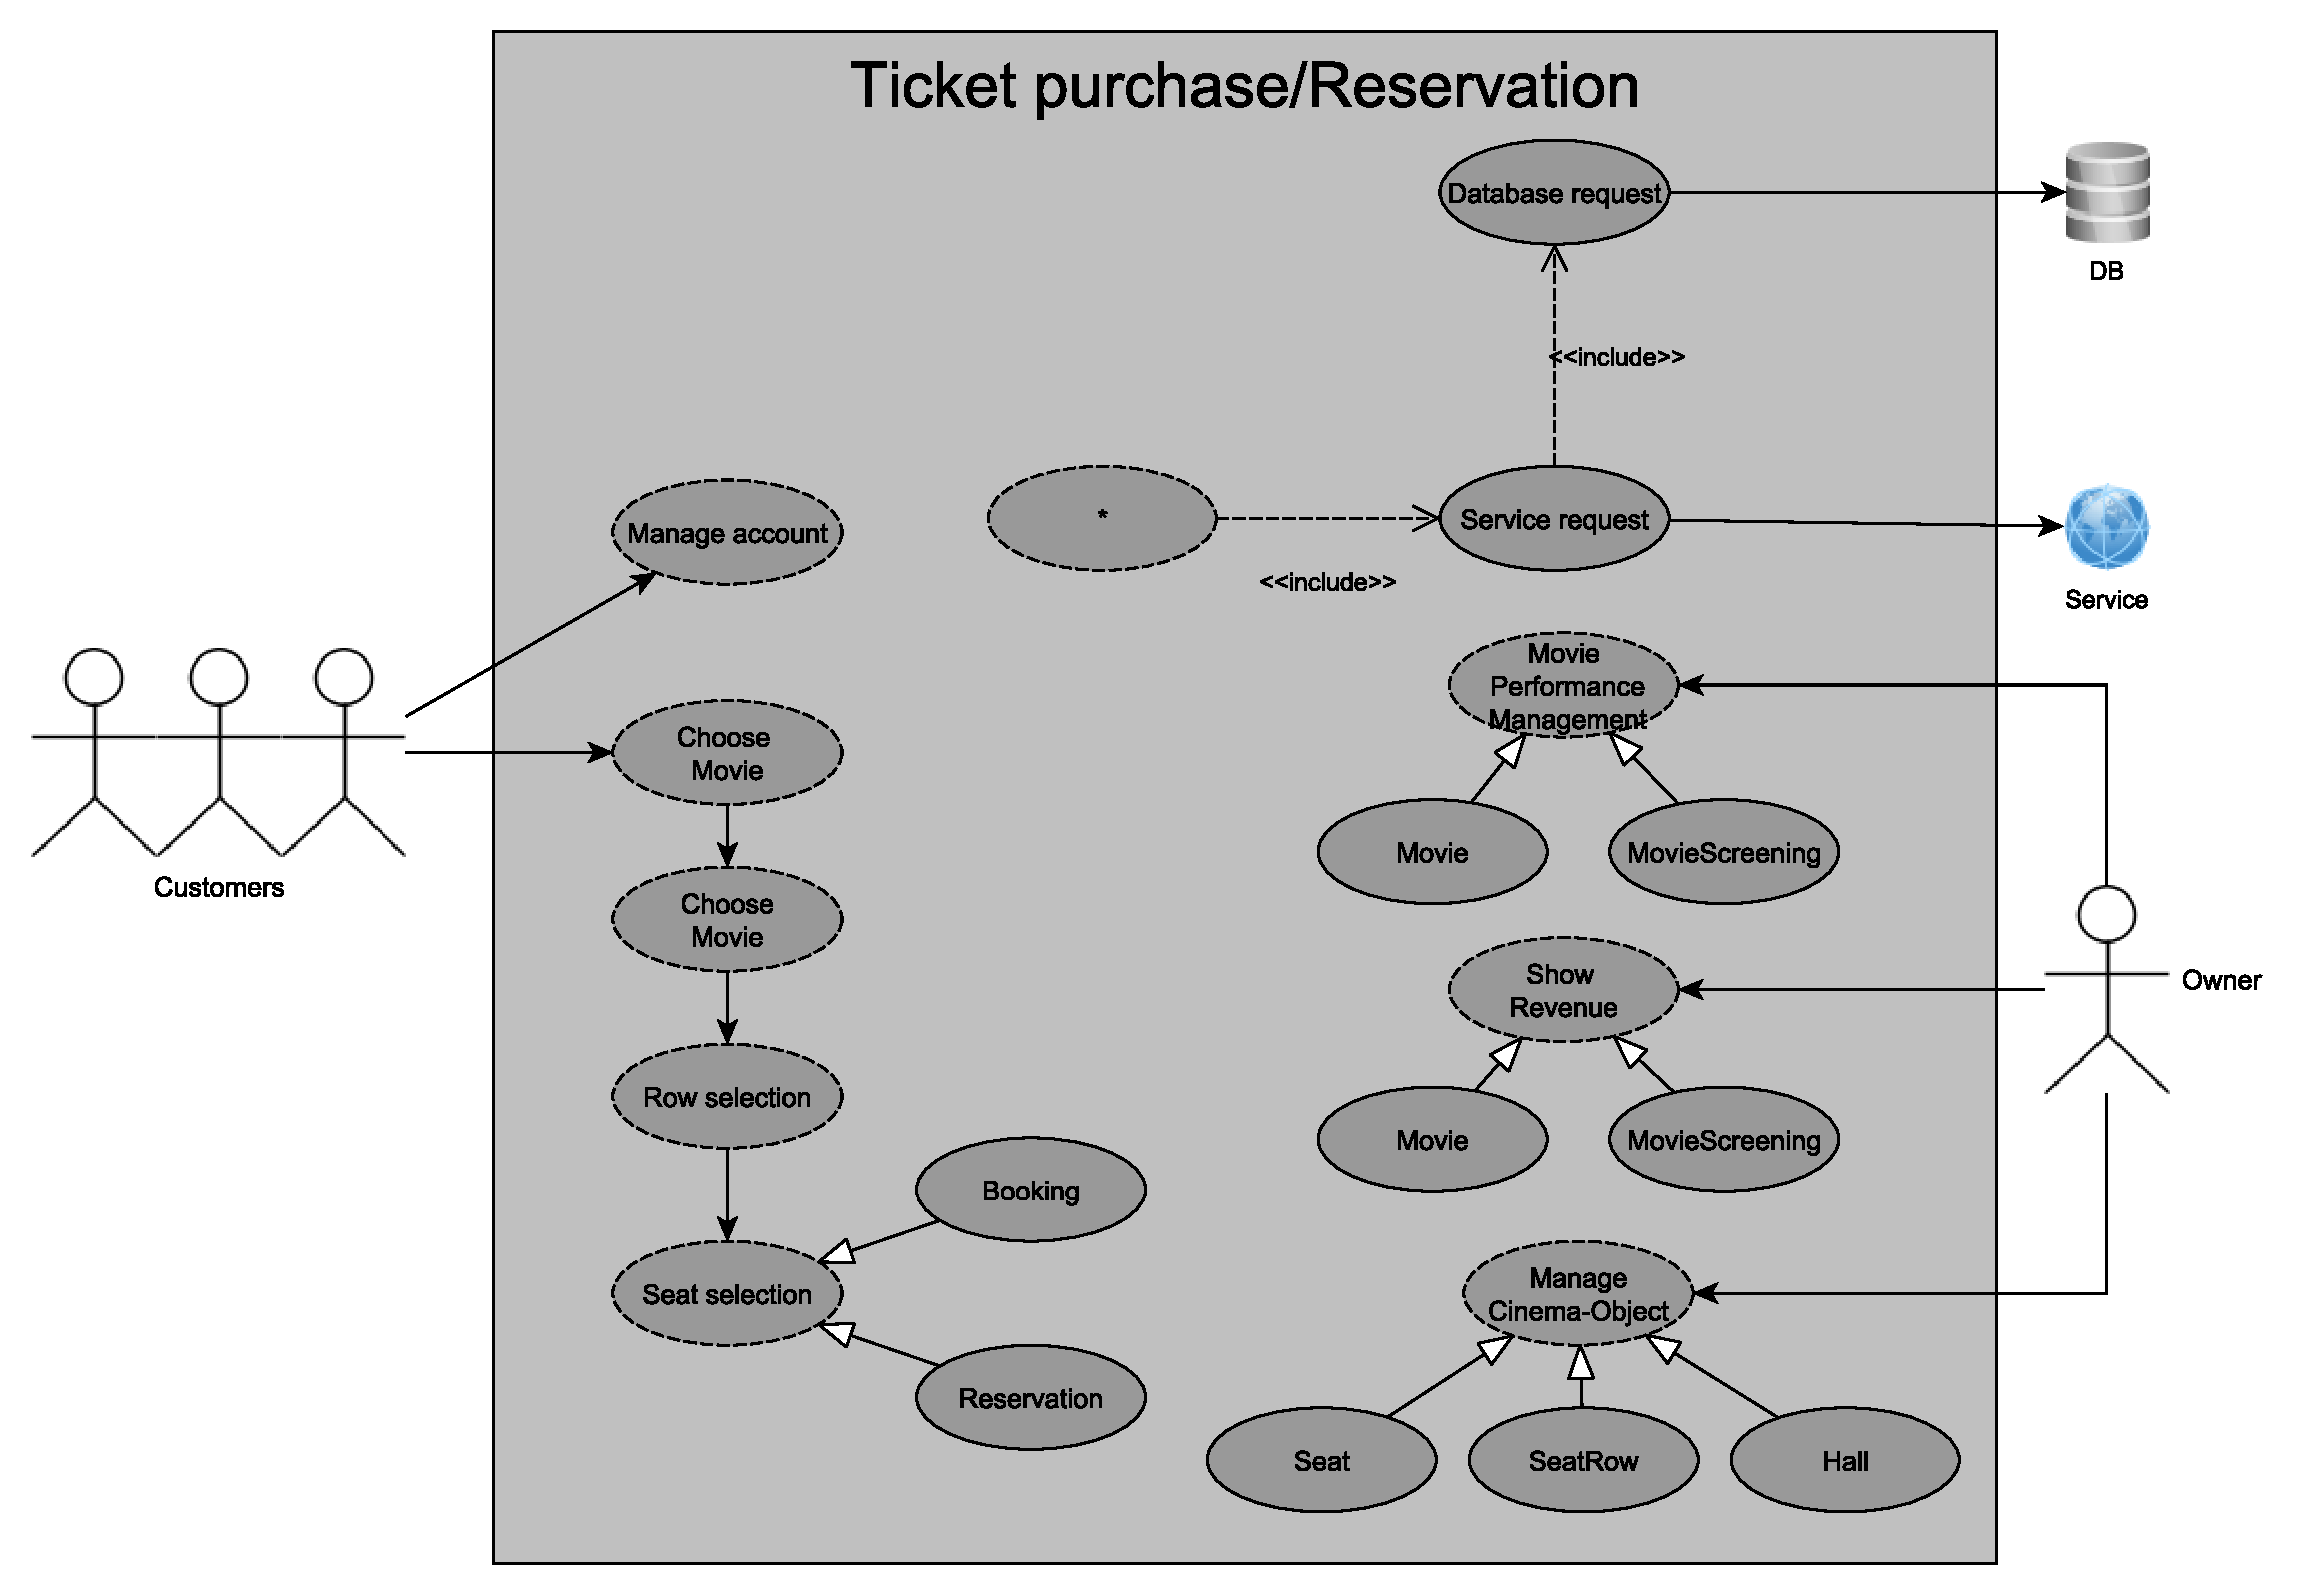
\includegraphics[width=\textwidth]{images/iis-use.case-new}
    \caption{Simplified use-case diagram of actor interaction with \gls{g:cms}.}
    \label{fig:use-cases}
\end{figure}

The simplified\footnote{To maintain brevity and clarity, activities involving \gls{a:api} requests have been indicated with dashed borders, rather than explicitly modeling \inlinecode{<<include>>} relationships. Nonetheless, the underlying semantics remain unchanged.} use-case diagram in Figure \ref{fig:use-cases} illustrates two primary interactions: one between the cinema owner and the proposed \gls{g:cms} solution, and the other between customers and the system.

The cinema owner can manage various aspects of the cinema through the \gls{g:cms}, including cinema halls, seats, seat rows, movies, and movie screenings. In this context, \enquote{manage} refers to the \gls{a:crud} operations. These cinema-infrastructure-related tasks are commonly denoted as \inlinecode{management} activities throughout this document. Additionally, the owner can view revenue generated from movies and individual screenings. These operations are categorized as administrative or \inlinecode{admin} use-cases.

Conversely, customers can create and manage accounts, reserve or book seats for movies, and view or cancel their reservations. They can select a movie, choose a specific screening, and pick their desired row and seat. Afterward, customers can either book the seat immediately or reserve it for booking later. The group of use-cases related to customer interactions is referred to as \inlinecode{user} use-cases.

While the diagram offers a fundamental overview of the \gls{g:cms} solution's desired functionality, it does not provide specific details. Consequently, the following section delves deeper into the technical implications of the various use-cases, deriving requirements accordingly.

A more detailed description of different scenarios and use-cases written in natural language is presented in \cref{apx:sec:use-cases}.

\section{Requirements}
\label{sec:requirements}

This section delves into the use-cases outlined in \cref{sec:use-cases}, with the aim of extracting requirements for a \gls{g:cms} prototype. To achieve this, the subsequent subsections examine the challenges and constraints associated with the various use-cases, along with their corresponding requirements.

\subsection{Interaction with \glsentrytext{g:cms}}\label{sec:req-interaction}
A fundamental question arising from the use-cases outlined in \cref{sec:use-cases} concerns the method of how an actor interacts with the proposed \gls{g:cms} solution. Specifically, whether a \gls{a:gui} or a \glsfull{a:cli} should be employed for system interaction. The primary distinction between these two approaches lies in \glspl{a:gui} utilizing visual cues to convey information to users, whereas \glspl{a:cli} rely on text-based commands for input and output of information.

The client has indicated that a full \gls{a:gui} is not required for the \gls{g:cms} prototype, suggesting that a \gls{a:cli} would suffice \cite[2]{IIS2-ass}. Nevertheless, considering that software solutions are often evaluated based on the user experience they offer, the development team has opted to prioritize delivering a user-friendly interface. This requirement entails that the \gls{g:cms} client application should be as accessible as a \gls{a:gui}, which can be accomplished by providing a \gls{a:cli} with a comprehensive feature set.

\subsection{Communication Between Actors and \glsentrytext{g:cms}}\label{sec:req-protocol}

Furthermore, the client specified that the \gls{g:cms} should be accessible to both the owner and customers through a client-server architecture \cite[2]{IIS2-ass}. As a result, it is essential to define the communication protocol to be employed by the \gls{g:cms} \gls{a:api}.

Apart from specifying network-based communication, no additional constraints have been imposed on the selection of the communication protocol. Consequently, the development team has opted to use the \gls{a:http} 1.1 specification, implementing a \gls{a:rest}ful \gls{a:api} that employs \gls{a:json} for data serialization. This choice is grounded in the widespread use of the \gls{a:rest} architecture for \glspl{a:api}, ensuring seamless interoperability with other software components that may extend the \gls{g:cms} solution in future development efforts. The decision for \gls{a:json} for data serialization is based on its status as a commonly used, standardized data-exchange format for \glspl{a:api}, increasing the likelihood of the client's familiarity with it. Additionally, its human-readable nature proves particularly valuable during development, facilitating easy debugging of the \gls{a:api}. Finally, as the \gls{a:json} format is a subset of the JavaScript language, which most web browsers natively support, it offers the potential for future development of a web-based user interface without necessitating extra dependencies \cite{rfc8259}.

\subsection{Client Portability}\label{sec:req-client-portability}

To guarantee a seamless user experience, the \gls{g:cms} client application must be accessible across various platforms, ensuring portability across operating systems and architectures. Ideally, it should be a standalone executable file without any additional dependencies.

Considering these requirements, the development team chose C\#/.NET as the programming language for the \gls{g:cms} client application. This decision was based on C\#/.NET's ability to be packaged as a self-contained executable file, enabling native compilation into architecture-specific binaries. Consequently, the client application can run on compatible systems without additional runtime or framework dependencies. The C\#/.NET ecosystem also offers a diverse set of libraries for \gls{a:cli}-development, such as \inlinecode{System.Commandline}, allowing for shorter development times and less boilerplate code for command parsing \cite{DotnetPublishing} \cite{DotnetPublishingAot}\cite{DotnetSystemCommandline}.

\pagebreak

\subsection{Summary of Requirements}
\label{sec:requirements-summary}

The investigation of the challenges elucidated in the use cases and the constraints associated therewith have led to the establishment of the following prerequisites for the proposed \gls{g:cms} solution. These requirements will serve as a basis for the conceptual design in the following chapter.

\renewcommand{\arraystretch}{1.25}
\begin{table}[H]
    \centering
    \caption{Summary of requirements for \gls{g:cms}.}
    \label{tab:requirements}
    \begin{tabular}{l|p{0.75\textwidth}}
        \toprule
        Requirement & Description \\ \midrule
        \requirementdefshort\label{req:use-cases}  & \gls{g:cms} must cover the use-cases discussed in \cref{sec:use-cases} and \cref{apx:sec:use-cases}. \\ \hline
        \requirementdefshort\label{req:model-requirements}  & \gls{g:cms} must comply with all model-specific requirements specified in \cref{apx:ch:extended-analysis}. \\ \hline
        \requirementdefshort\label{req:client-server} & \gls{g:cms} must utilize the client-server architecture, allowing multiple concurrent clients to access its services \cite[2]{IIS2-ass}. \\ \hline
        \requirementdefshort\label{req:database} & A database engine must be used to persist cinema data. \\ \hline
        \requirementdefshort\label{req:server} & The \gls{g:cms} server must be written in as a Java application complying with the principles of \gls{a:mdd} \cite[1]{IIS2-ass}. \\ \hline
        \requirementdefshort\label{req:mps} & \gls{a:mps} by JetBrains must be used to generate the Java source code for data access layer and the \gls{a:sql} \gls{a:ddl} statements required for the database schema \cite[1]{IIS2-ass}. \\ \hline
        \requirementdefshort\label{req:mysql} & \gls{g:cms} data must be persisted in a MySQL database \cite[4]{IIS2-ass}. \\ \hline
        \requirementdefshort\label{req:isolation} & Database access must be performed in a thread-safe and isolated manner \cite[2]{IIS2-ass}. \\ \hline
        \requirementdefshort\label{req:api} & The server must provide a \gls{a:rest}ful \gls{a:json} \gls{a:api} for the client application to communicate with, as established in \cref{sec:req-protocol}. \\ \hline
        \requirementdefshort\label{req:client-access} & The client application must be able to connect to the server via a \gls{a:rest}ful \gls{a:json} \gls{a:api} using \gls{a:http} 1.1 as the underlying protocol (see \cref{sec:req-protocol}). \\ \hline
        \requirementdefshort\label{req:client-cli} & A \gls{a:cli} must be provided for user interaction within the client application, as established by \cref{sec:req-interaction}. \\ \hline
        \requirementdefshort\label{req:client-firendly-cli} & Although a \gls{a:cli} is sufficient for the prototype, usability and user experience should be a priority for the development, as established by \cref{sec:req-interaction}. \\ \hline
        \requirementdefshort\label{req:client-portability} & The client application must be capable of being published as a self-contained executable, guaranteeing portability without reliance on any additional runtime environment for installation. This requirement was established in \cref{sec:req-client-portability} \\ 
        \bottomrule
    \end{tabular}
\end{table}
\renewcommand{\arraystretch}{1}
\chapter{Conceptual solution}
\label{ch:concept}

This chapter introduces the proposed conceptual solution, which forms the basis for the implementation discussed in \cref{ch:impl}. Initially, an overview of the project structure is provided. Subsequently, the server-side infrastructure is examined, assessing the most suitable data model for use with \gls{a:mps} code generation, emphasizing key components, and ensuring thread-safe interactions among them. Finally, the client application is explored in depth, addressing its architecture, design, and quality of life enhancements.

\section{Project Infrastructure}\label{sec:infrastructure}

This section introduces the architectural solution designed to meet the requirements delineated in \cref{sec:requirements}. The comprehensive project architecture is illustrated in \cref{fig:architecture}, which encompasses three primary components: the client application, the server-side infrastructure, and the database.
\vspace{-.2cm}
\begin{figure}[H]
    \centering
    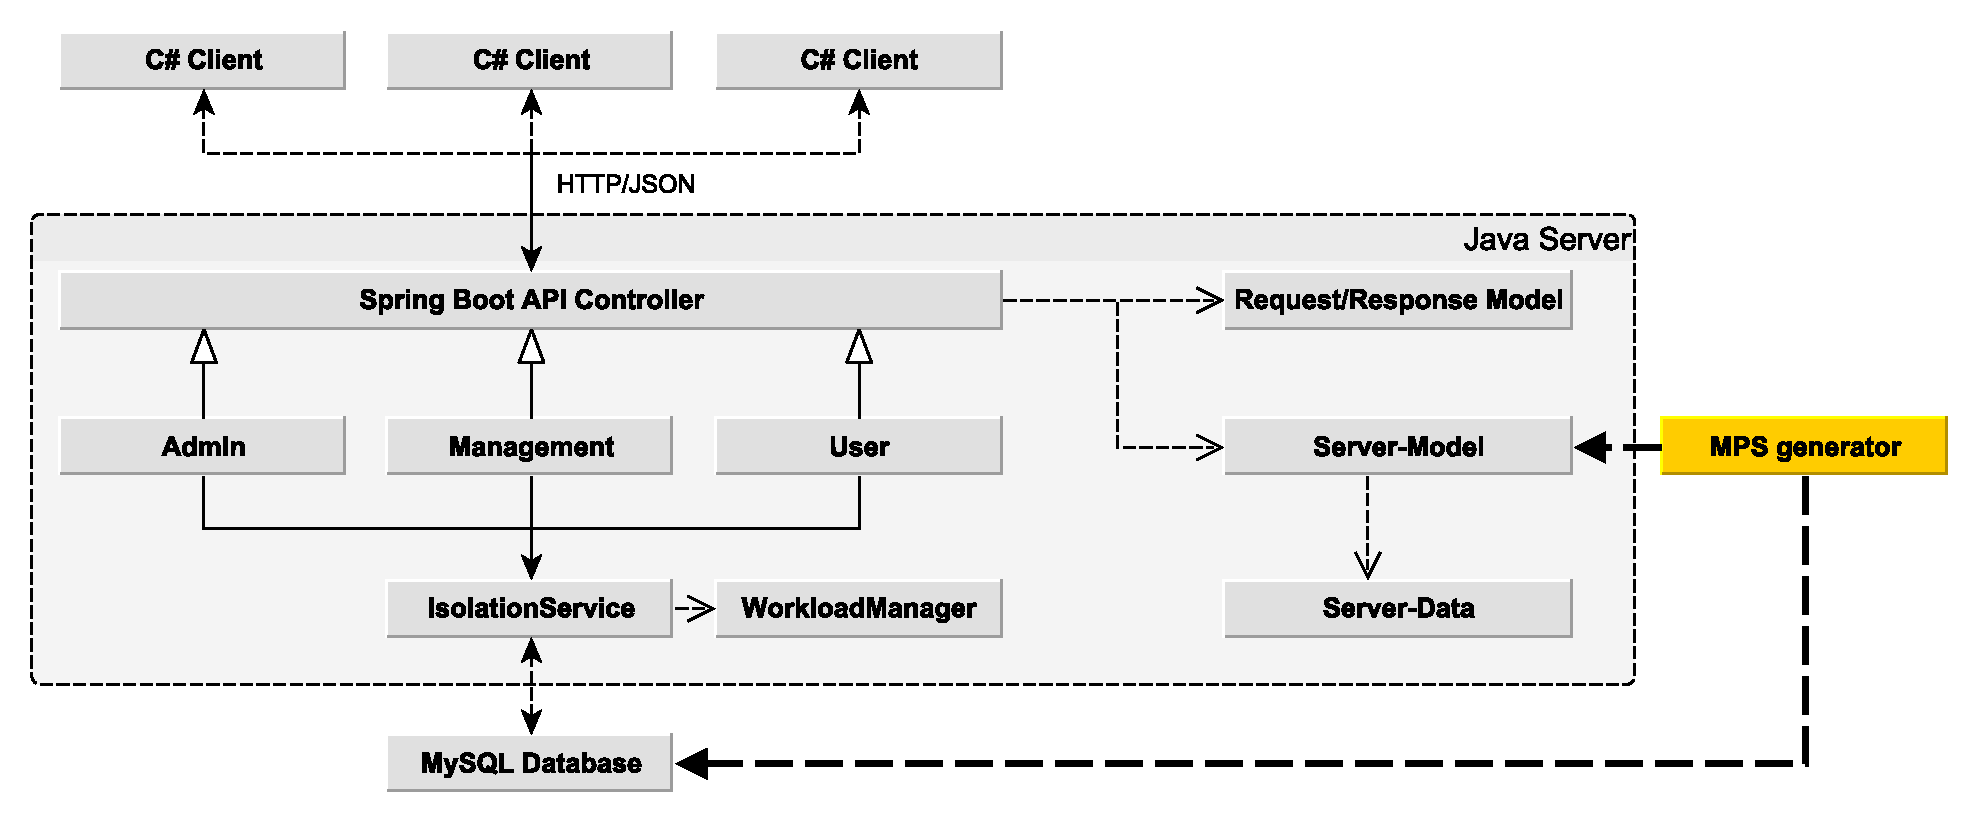
\includegraphics[width=\textwidth]{images/big-picture-no-lombok}
    \caption{Key aspects encompassing project architecture of the proposed solution.}
    \label{fig:architecture}
\end{figure}
\vspace{-.35cm} % :)
\Cref{fig:architecture} illustrates the project architecture for the proposed solution. The architecture allows for multiple client application instances to connect concurrently to a single server instance, facilitating simultaneous user interactions. Communication between the client and server is achieved through a \gls{a:rest}ful \gls{a:json} \gls{a:api}, which adheres to standardized conventions and promotes interoperability between the C\# clients and the Java server. The design of the client is elaborated in further details in \cref{sec:cs-client}.

Upon invoking a specific endpoint using the client application, the server-side \gls{g:spring} \gls{a:api} controllers handle deserialization of the corresponding \gls{a:json} request model in accordance to the \gls{a:api} design specified in \cref{sec:cs-api}. These \gls{a:api} controllers subsequently process the request utilizing the \gls{a:mps}-generated data access layer elucidated in \cref{sec:cs-data-model}, therefore ensuring a consistent, efficient, and maintainable interface with the underlying data storage.

The \inlinecode{IsolationService} plays a crucial role in managing and scheduling the data access requests performed by the \gls{a:api} controllers. It provides a level of isolation between concurrent requests, ensuring data consistency and preventing conflicts or race conditions. This service facilitates communication with the \gls{a:mps}-generated database schema, which is tailored to efficiently store and manage the system's data. A more comprehensive overview of the isolation service is provided in \cref{sec:cs-isolation}.
\vspace{-.15cm} % :)

\section{Server}

The server application constitutes the central component of the \gls{g:cms}, overseeing the data model management and furnishing a \gls{a:rest} \gls{a:api} for client interactions. The implementation of the data model harnesses the \gls{a:mps} framework, while the \gls{a:rest} \gls{a:api} employs the \gls{g:spring} framework. Developed using Java, the server application capitalizes on the Maven build system. Ensuing sections provide a thorough analysis of the server application's architecture, commencing with an overview of the data model derived from the use-cases delineated in \cref{sec:use-cases}, continuing with an exposition of the \gls{a:rest} \gls{a:api}, and concluding with the presentation of the isolation layer.

\subsection{Data Model Design}\label{sec:cs-data-model}

To adhere to the requirements identified in \cref{ch:problem-analysis} and \cref{apx:ch:extended-analysis}, a data model has been designed, as illustrated in \cref{fig:data-model}. The data model represents the essential entities and their relationships within the \gls{g:cms} domain.
\vspace{-.25cm} % :)

\begin{figure}[H]
    \centering
    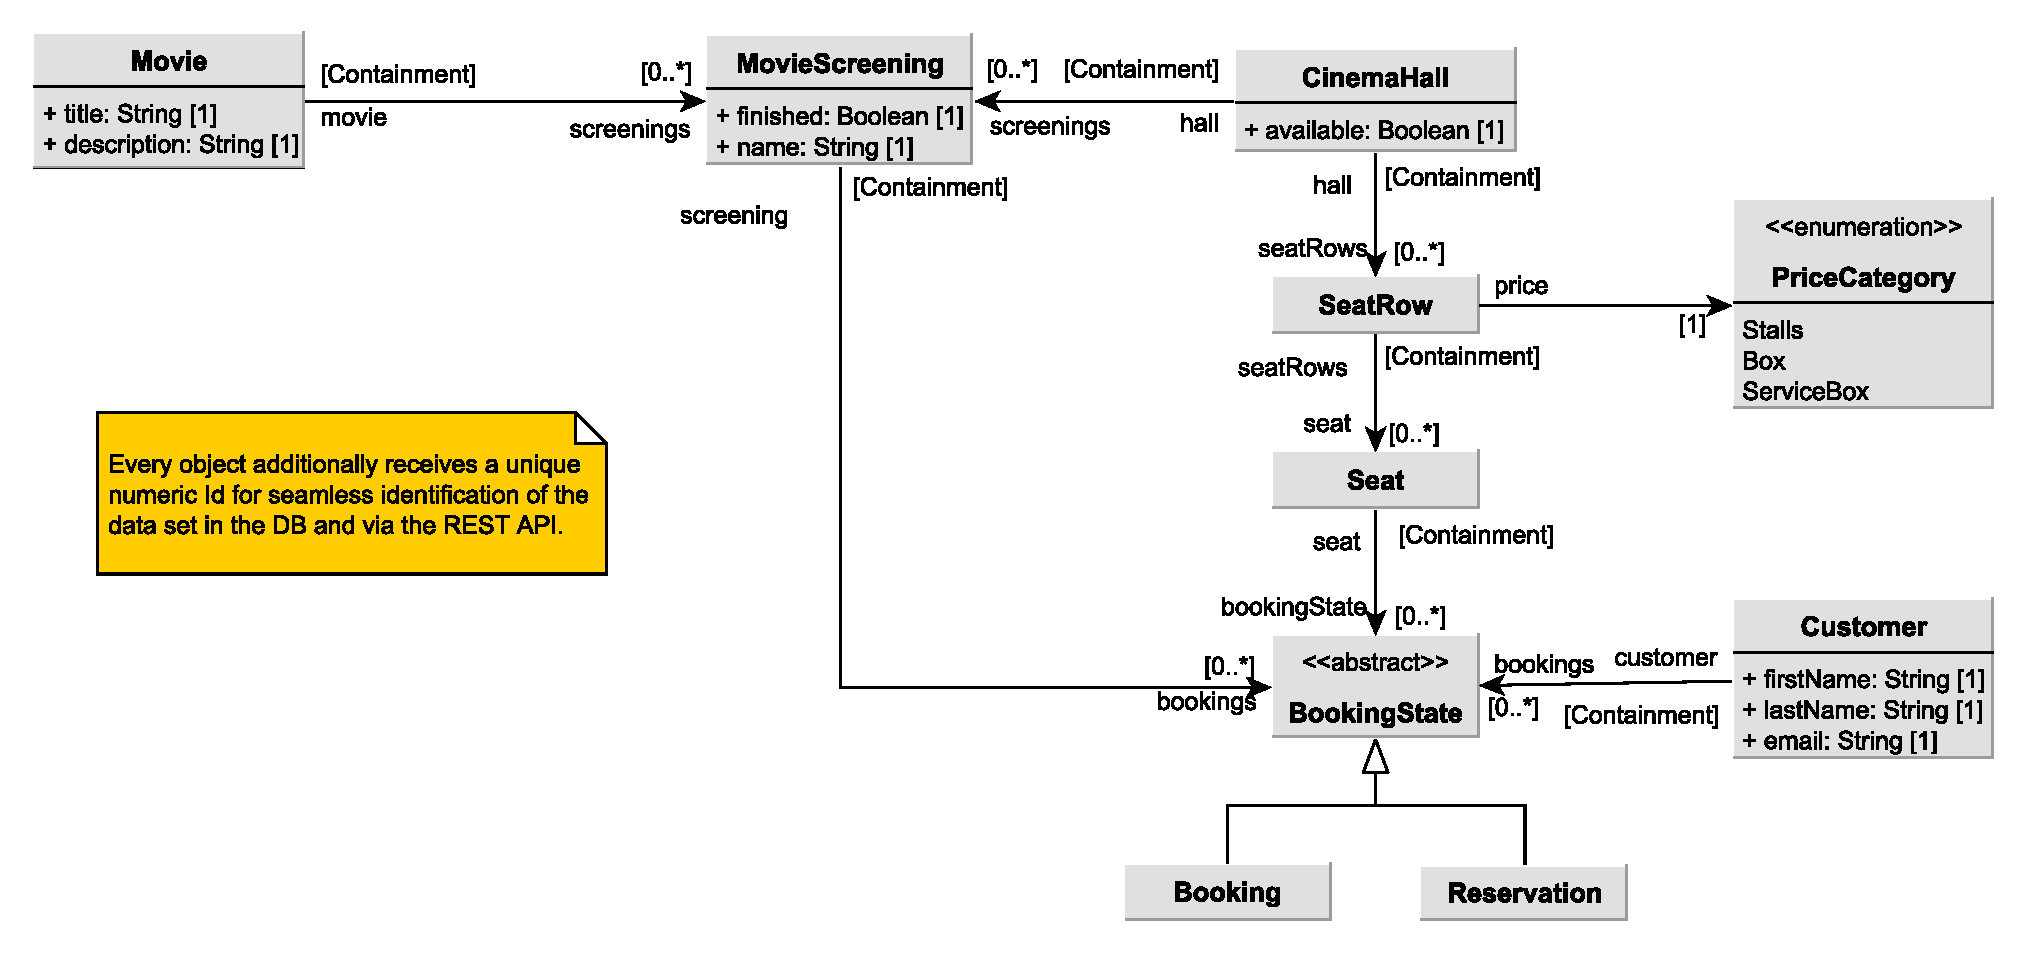
\includegraphics[width=\textwidth]{images/data-model-final-enum}
    \caption{Data model for \gls{g:cms} according to requirements.}
    \label{fig:data-model}
\end{figure}

To formally prove the correctness of the proposed data model depicted in \cref{fig:data-model}, the validity of all relationships within the model must be ensured. The following definitions apply to an association between two classes $A$ and $B$, represented by a function $R : A \to B$:

\begin{description}[labelwidth=\linewidth, listparindent=0pt]
    \item[Partial function]\phantomsection\label{def:partial}
        $R$ is a partial function if and only if the following holds true:
        $$\forall (x_1, x_2), (x_1', x_2')\in R : x_1 = x_1' \implies x_2 = x_2'$$
        In other words: \enquote{Every instance of $A$ owns at most one $B$ object}.
    \item[Total function]\phantomsection\label{def:total}
        $R$ is a total function if and only if the following holds true: $R$ is a partial function and
        $$\forall x_1 \in A: \exists x_2 \in B: (x_1, x_2) \in R$$
        In other words: \enquote{Every instance of $A$ owns exactly one $B$ object}.
    \item[Injective function]\phantomsection\label{def:injective}
        $R$ is an injective function if and only if the following holds true:
        $$\forall (x_1, x_2), (x_1', x_2')\in R : x_2 = x_2' \implies x_1 = x_1'$$
        In other words: \enquote{Every $A$ object is uniquely identifiable using the associated instance of $B$} or \enquote{Given an instance of $B$, the corresponding $A$ object is uniquely identifiable}.
    \item[Surjective function]\phantomsection\label{def:surjective}
        $R$ is a surjective function if and only if the following holds true:
        $$\forall x_2 \in B: \exists x_1 \in A: (x_1, x_2) \in R$$
        In other words: \enquote{Any $B$ object can not exist without a corresponding instance of $A$} or \enquote{$B$ is entirely dependent on $A$}. 
    \item[Containment]\phantomsection\label{def:containment}
        $R$ is a containment if and only if the following holds true: $R$ is an injective and surjective function.
        
        In other words: \enquote{Given an instance of $B$, the corresponding $A$ object is uniquely identifiable. Additionally the $B$ object can not exist without a corresponding instance of $A$}.
\end{description}

On the following page these properties are proven for every association in \cref{fig:data-model}.

\pagebreak

For the convenience of the reader, \cref{fig:data-model} is repeated below.
\vspace{-.2cm}
\begin{figure}[H]
    \centering
    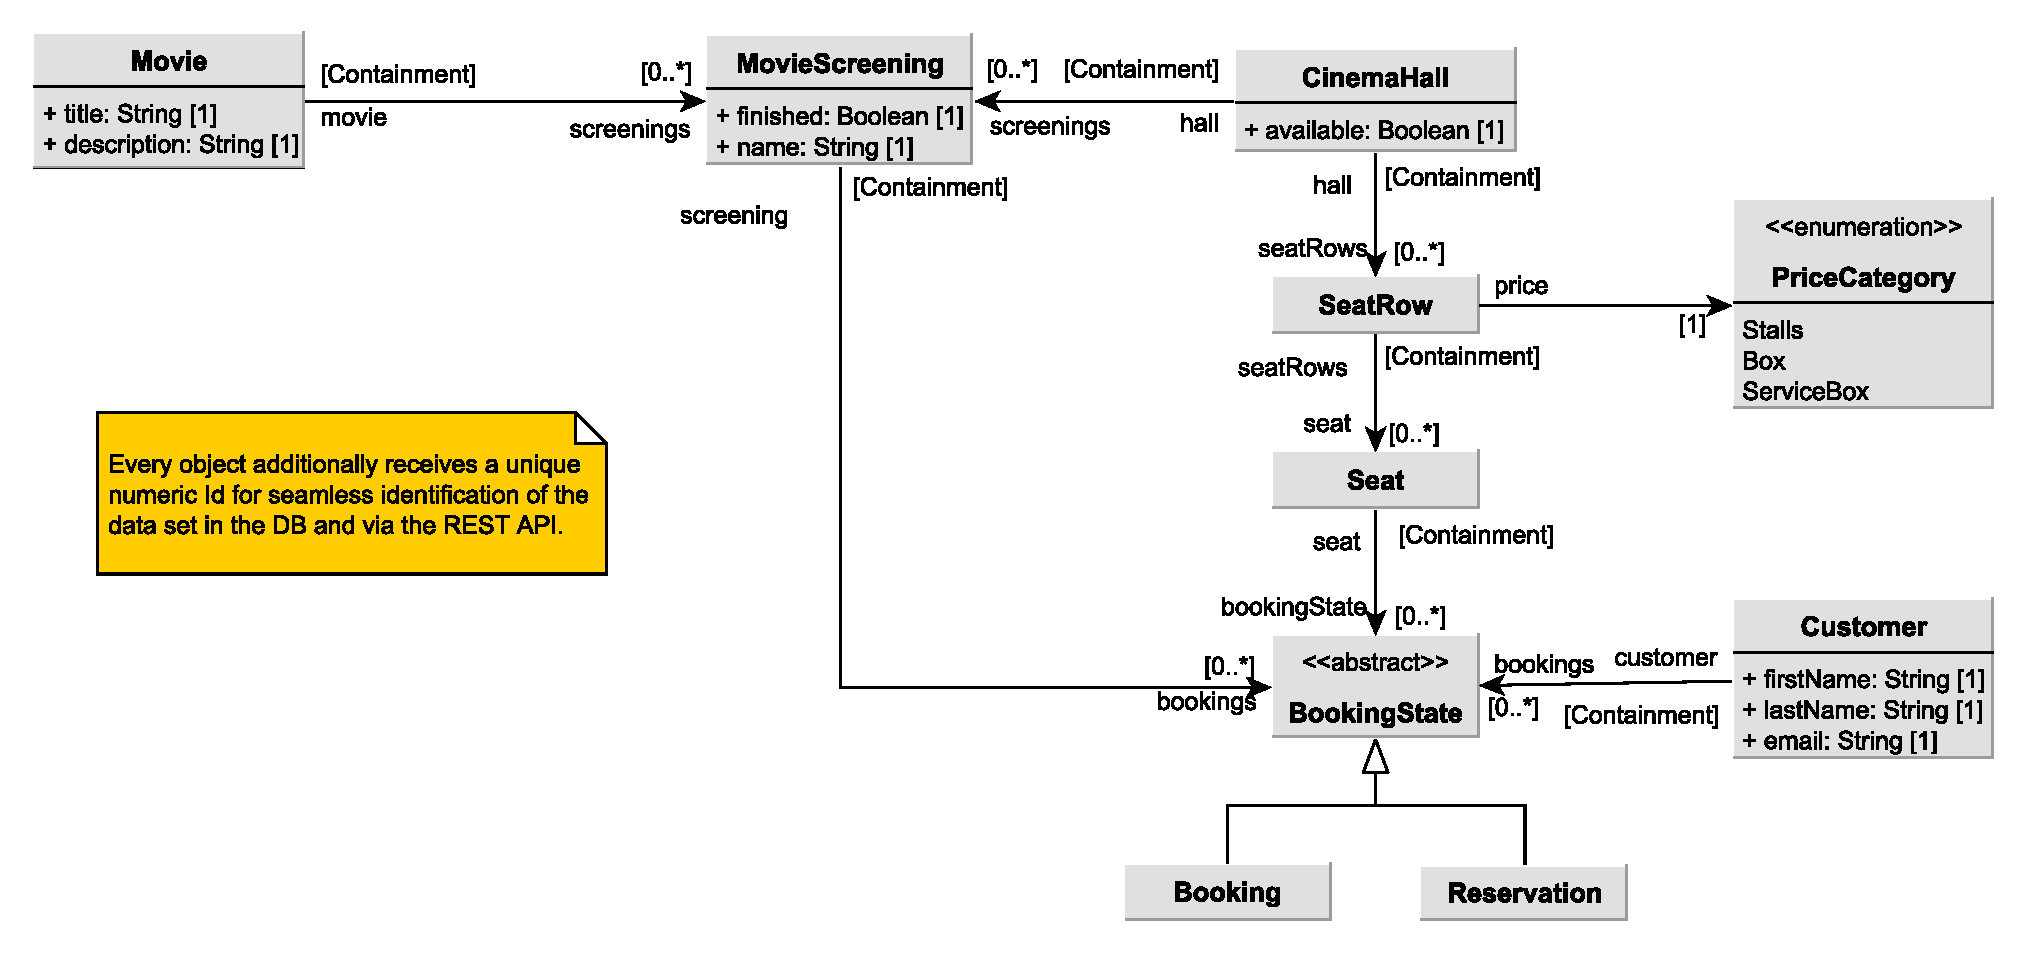
\includegraphics[width=0.9\textwidth]{images/data-model-final-enum}
\end{figure}
\vspace{-.6cm}

The class \inlinecode{Movie} comprises two attributes: a title and a description, both represented as strings. The \inlinecode{MovieScreening} class includes two attributes as per the requirements: a boolean attribute named \inlinecode{finished} indicating whether the movie screening has already taken place, and a string attribute called \inlinecode{name} allowing a human-readable representation of the screening to be stored.

The association from \inlinecode{Movie} to \inlinecode{MovieScreening} implies that every \inlinecode{Movie} is unambiguously identifiable given a \inlinecode{MovieScreening} instance. A \inlinecode{MovieScreening} without a corresponding \inlinecode{Movie} would be meaningless, making the association a \containment.

Moreover, for every \inlinecode{MovieScreening} a \inlinecode{CinemaHall} class is required (\surjectivity) and given a screening, the hall must be unambiguously identifiable (\injectivity $\implies$ \containment). The cinema hall features a single attribute to denotes whether the hall is available for being used to create movie screenings.

The data model also includes a class called \inlinecode{SeatRow}, with a corresponding \inlinecode{PriceCategory}, and another class called \inlinecode{Seat}. The \inlinecode{CinemaHall} class and the \inlinecode{SeatRow} class have a \containment association, as a seat row cannot practically exist without a hall, and there can only be one hall per seat row. Another \containment association exists from \inlinecode{SeatRow} to \inlinecode{Seat}, because for the context of cinema management, a seat without an associated row is pointless, additionally, given a seat the corresponding row should be clearly determinable.

Moreover, the booking system necessitates an abstract class, \inlinecode{BookingState}, which is further refined by the \inlinecode{Reservation} and \inlinecode{Booking} classes. A \containment association exists between the \inlinecode{Seat} class and the abstract \inlinecode{BookingState} class, as a booking state (ticket) must always be associated with a seat and uniquely identify it. The \inlinecode{MovieScreening} class has a second \containment association with \inlinecode{BookingState}, signifying that a ticket is entirely dependent on a movie screening and can be used for unambiguous identification of the screening.

Lastly, the \inlinecode{Customer} class embodies the cinema's patrons and encompasses three attributes: first name, last name, and email address. An association exists between the \inlinecode{Customer} and \inlinecode{BookingState} (ticket) classes to distinctly associate each customer with their respective bookings. Since a \inlinecode{BookingState} cannot exist without a customer, this relationship is also considered a \containment.

\subsubsection{Compliance with MPS}\label{sec:cs-data-mps}

Due to technical constraints imposed by \gls{a:mps}, the data model introduced in \cref{fig:data-model} necessitated adjustments prior to implementation.

\Cref{fig:data-model} specified an enumeration for representing price categories within the data model, which is not easily modeled within \gls{a:mps}. Consequently, for database representation, an abstract class with sub-classes was employed to improve maintainability and extensibility compared to a flat integer or string representation. As such, the class diagram in \cref{fig:data-model-mps} was specified in order to reflect these changes.

\begin{figure}[H]
    \centering
    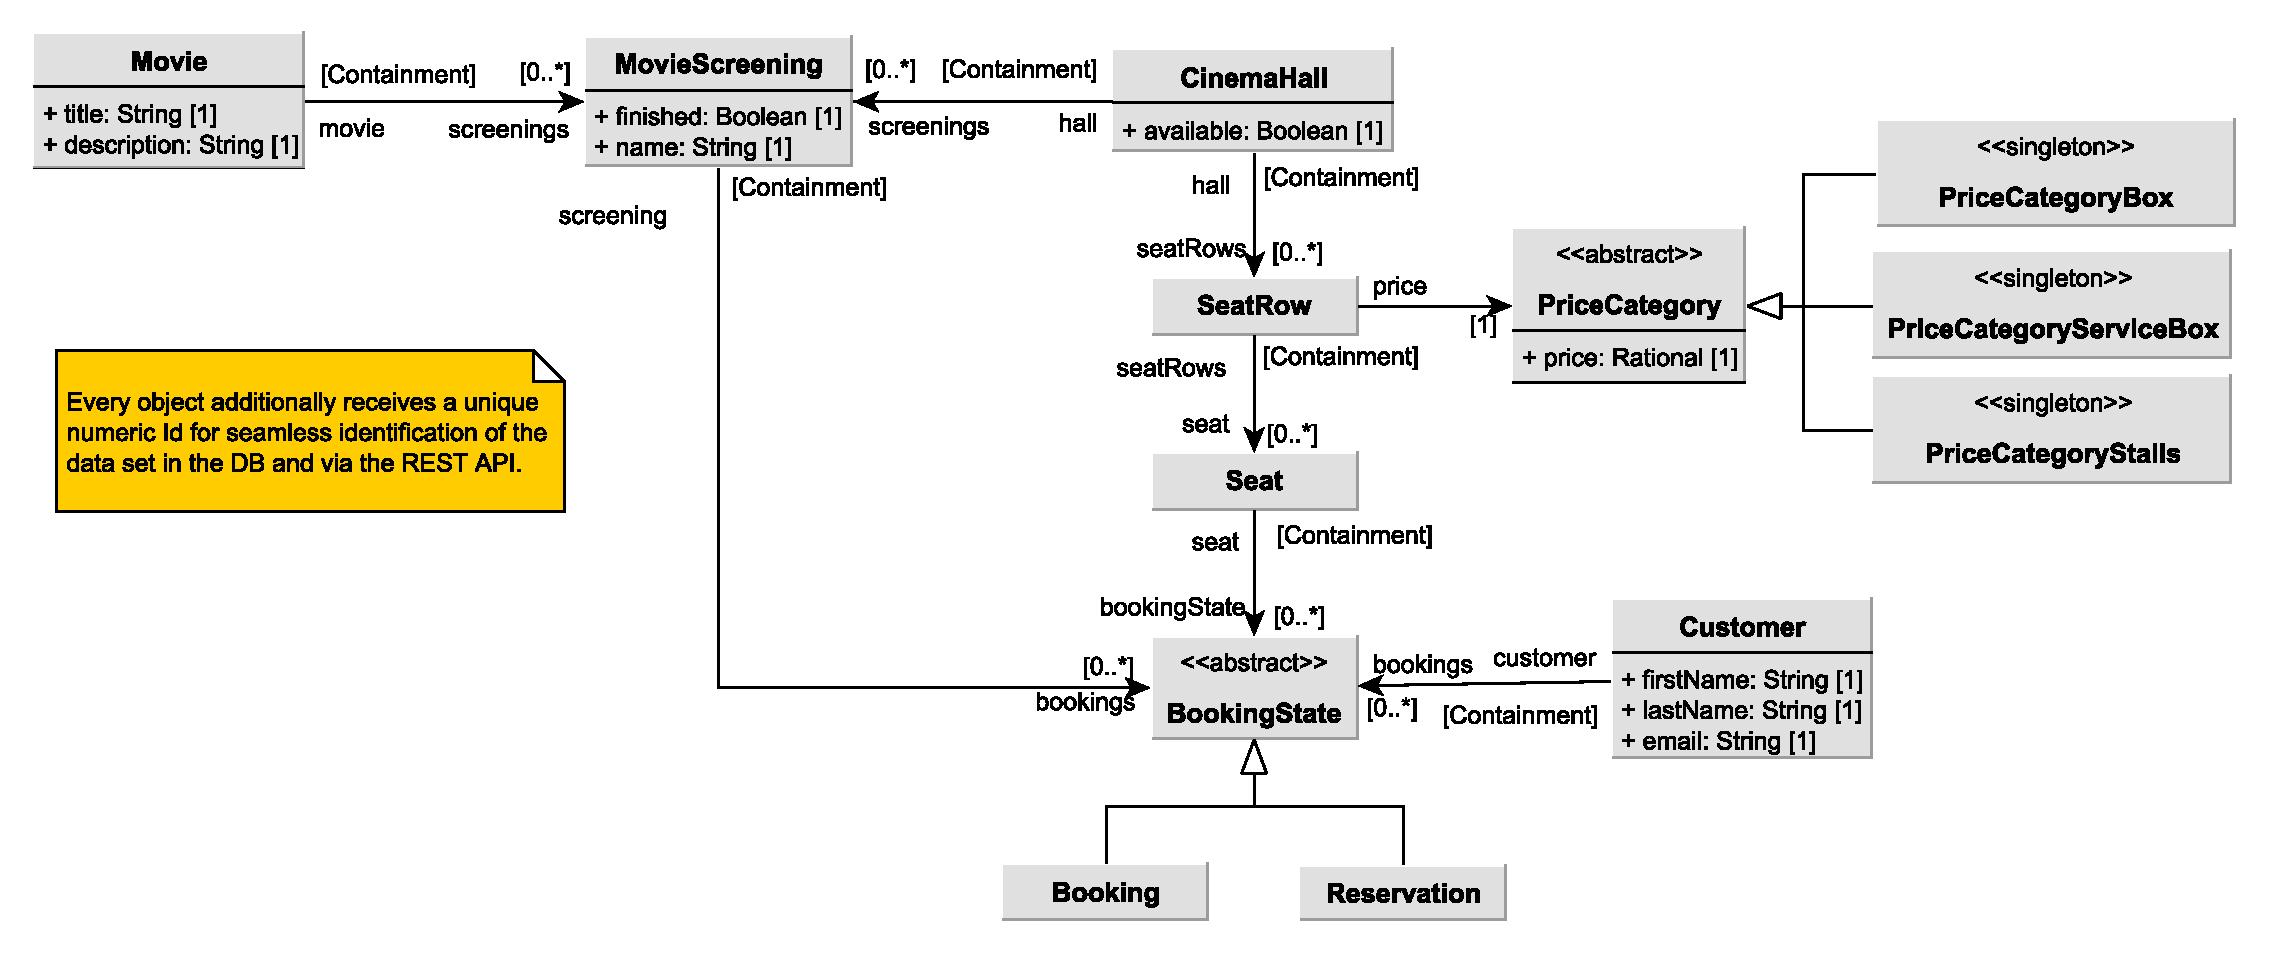
\includegraphics[width=\textwidth]{images/data-model-final-with-price}
    \caption{Adjusted data model for \gls{g:cms} due to technical limitations.}
    \label{fig:data-model-mps}
\end{figure}

As depicted in \cref{fig:data-model-mps}, the \inlinecode{PriceCategory} enumeration has been replaced by an abstract class comprising three singleton subclasses: \inlinecode{PriceCategoryBox} for the \inlinecode{Box} price category, \inlinecode{PriceCategoryServiceBox} for the \inlinecode{ServiceBox} price category, and \inlinecode{PriceCategoryStalls} for the \inlinecode{Stalls} price category.

Transitioning from an enumeration to an abstract class with inheriting singletons offers several advantages. First, it enhances type safety by mitigating potential risks of invalid changes to data associated with using flat integers or string representations in the database. Singleton classes guarantee a single instance of each concrete price category, minimizing errors due to inconsistent states. Furthermore, employing abstract classes and inheritance fosters better code organization.

Another benefit of this modification is the ability to directly incorporate price values within new price category classes. As such, the \inlinecode{price} attribute was added as a \inlinecode{Rational} number.

\pagebreak

\subsection{REST API}\label{sec:cs-api}

The \gls{a:rest} \gls{a:api} offers the client application an interface for interacting with the server. It comprises a set of \gls{a:rest}ful \gls{a:json} \gls{a:api} endpoints, with each endpoint handling a specific task.

\subsubsection{Endpoint Design}\label{sec:cs-api-endpoints}

To achieve a consistent and intuitive \gls{a:api} design, the endpoints were developed based on the use-cases outlined in \cref{sec:use-cases}. Consequently, the endpoints are initially grouped by the role responsible for performing the action, followed by the target of the action, and finally by the action itself. \Cref{fig:api-tree} illustrates a portion of the resulting tree structure of the \gls{a:api} endpoints, which is subsequently employed to create the Java \gls{g:spring} controllers.

\begin{figure}[H]
\renewcommand*\DTbaselineskip{10pt}
{\scriptsize
\dirtree{%
.1 \apiexpanded \ /.
.2 \apiexpanded management/. 
.3 \apicollapsed cinema-hall/ \apihandledby \syntaxcomplex{CinemaHallController}.
.3 \apiexpanded movie/ \apihandledby \syntaxcomplex{MovieController}.
.4 list \type \syntaxprimitive{GET} \apihandledby listMovies() \type \syntaxkeyword{GetMoviesResponse}.
.4 list-full \type \syntaxprimitive{GET} \apihandledby listDetailedMovies()\type \syntaxkeyword{GetMoviesFullResponse}.
.4 create \type \syntax[colorbrownish]{POST} \apihandledby createMovie(\syntaxkeyword{CreateMovieRequest})\type \syntaxkeyword{CreateMovieResponse}.
.4 update \type \syntax[colorbrownish]{POST} \apihandledby updateMovie(\syntaxkeyword{UpdateMovieRequest})\type \syntaxkeyword{UpdateMovieResponse}.
.4 delete \type \syntax[colorbrownish]{POST} \apihandledby deleteMovie(\syntaxkeyword{DeleteMovieRequest})\type \syntaxkeyword{DeleteMovieResponse}.
.3 \apicollapsed movie-screening/ \apihandledby \syntaxcomplex{MovieScreeningController}.
.3 \apicollapsed seat/ \apihandledby \syntaxcomplex{SeatController}.
.3 \apicollapsed seat-row/ \apihandledby \syntaxcomplex{SeatRowController}.
.2 \apiexpanded user/.
.3 \apicollapsed account/ \apihandledby \syntaxcomplex{UserAccountController}.
.3 \apicollapsed booking/ \apihandledby \syntaxcomplex{UserBookingController}.
.2 \apiexpanded admin/.
.3 \apicollapsed revenue/ \apihandledby \syntaxcomplex{AdminController}.
}
}
\renewcommand*\DTbaselineskip{20pt}
\raggedleft
{\scriptsize\vspace{-1cm}
\begin{tabular}{r@{ $\equalhat$ }l r@{ $\equalhat$ }l}
    \apicollapsed & \enquote{group collapsed} & \apiexpanded & \enquote{group expanded}\\
    \type & \enquote{is of type} & \apihandledby & \enquote{is handled by}\\
    \syntax[colorprimitive]{GET} & \enquote{\glsshort{a:http} GET request} & \syntax[colorbrownish]{POST} & \enquote{\glsshort{a:http} POST request}
\end{tabular}
\vspace{.25cm}}
\caption{Excerpt of the \gls{a:api} tree structure.}
\label{fig:api-tree}
\end{figure}

\Cref{fig:api-tree} presents an overview of all \gls{a:api} controllers and specifically of the endpoints within the \inlinecode{/management/movie} group. The \gls{a:api} endpoints are initially divided into three logical groups: \inlinecode{management}, \inlinecode{user}, and \inlinecode{admin}, each representing a different role. These logical groupings correspond to the Java packages containing the \gls{g:spring} controllers. On the second level, the endpoints are organized by their target, such as \inlinecode{movie} or \inlinecode{cinema-hall} for the management group. This second level maps to the respective Java \gls{g:spring} controller. Lastly, on the third level, endpoints are defined to handle the corresponding action, such as \inlinecode{list} or \inlinecode{create} for the movie controller. These endpoints map to the equivalent Java \gls{g:spring} controller methods.

Depending on the parameters necessary for executing the request action, either \inlinecode{GET} or \inlinecode{POST} requests are utilized. This is attributed to the fact that only \inlinecode{POST} requests can accommodate a body containing a \gls{a:json}-serialized request model. Consequently, communication through the \gls{a:api} is consistently \gls{a:json}-based, thereby complying with \cref{req:api}. This approach simplifies the communication process, as both the client and server can effortlessly serialize and deserialize \gls{a:json} data, provided the \glspl{a:rrm} correspond. Additionally, \gls{a:json} is a prevalent choice for \gls{a:rest} \glspl{a:api} due to its lightweight nature, human readability, and compatibility with most programming languages, ensuring technology independence \cite{rfc8259}.

Java \gls{g:spring} controllers are tasked with converting \gls{a:json} request data into their respective Java request models and transforming Java response models into \gls{a:json} response data. To avert tight coupling and unintended cross-dependencies, each \gls{a:rrm} is exclusively employed by a single \gls{a:api} endpoint, facilitating model modification without the need for considering other endpoints. This encapsulation is illustrated in the simplified class diagram presented in \cref{fig:api-controllers}.

\begin{figure}[H]
\centering
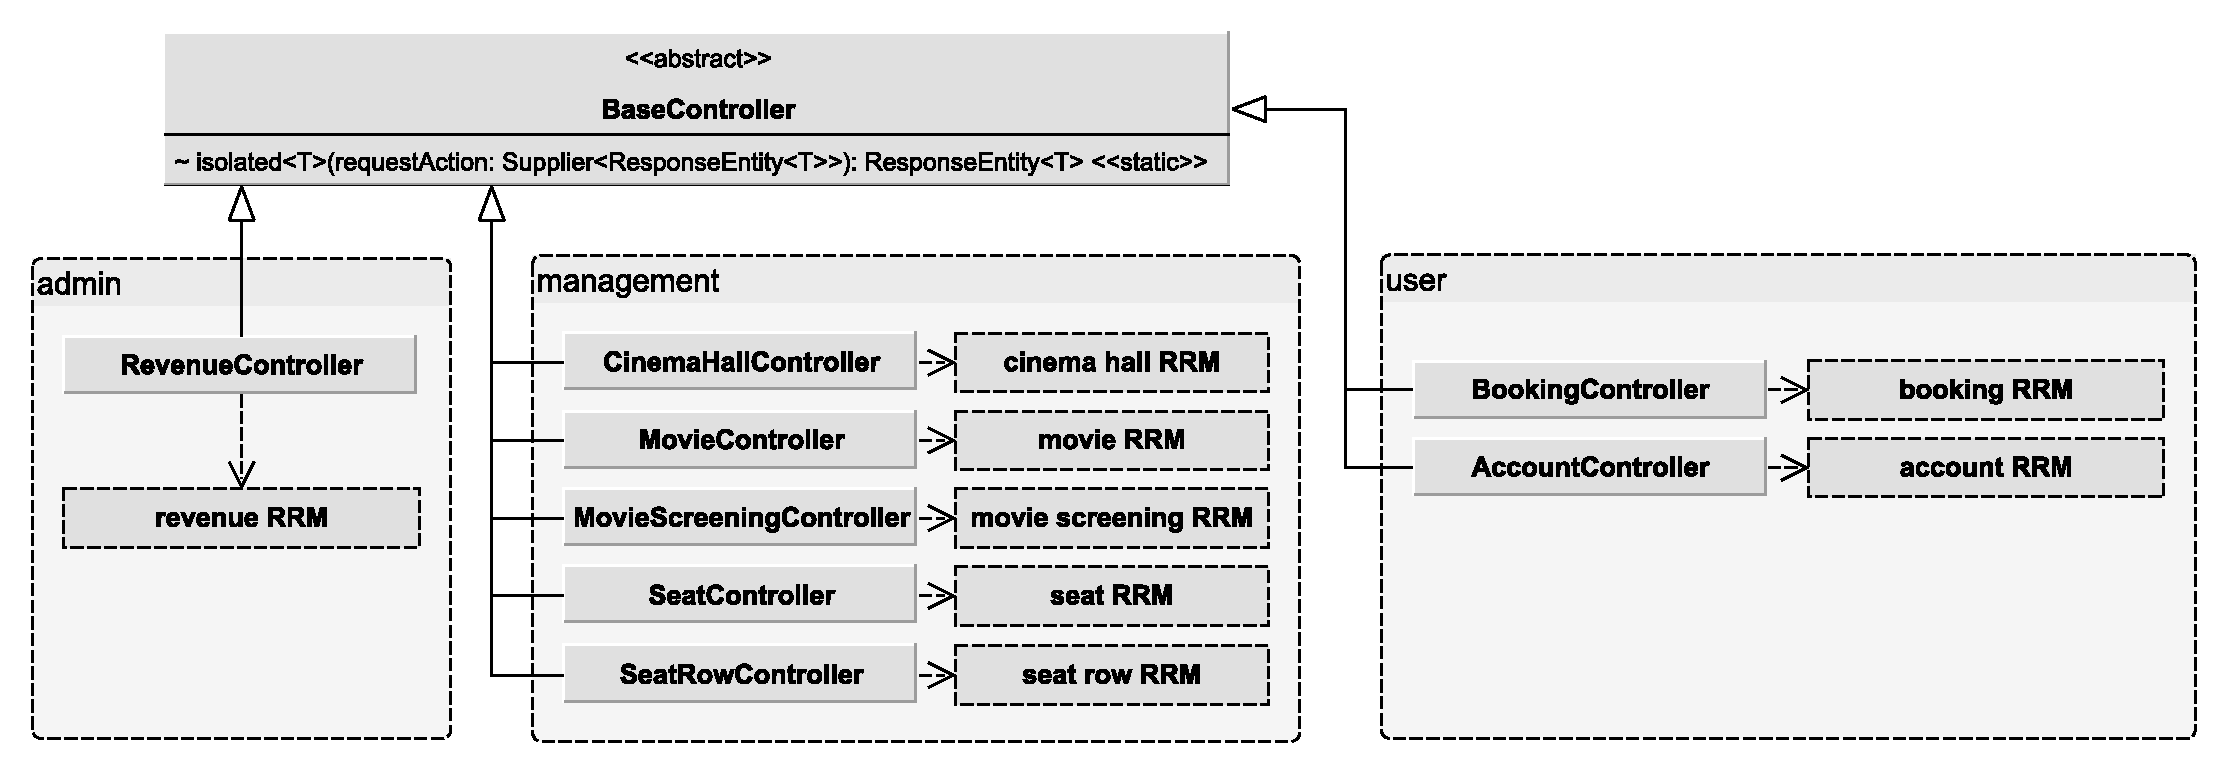
\includegraphics[width=\textwidth]{images/api-controllers}
\caption{Simplified \gls{a:api} controller structure with encapsulated \glspl{a:rrm}.}
\label{fig:api-controllers}
\end{figure}

However, the \gls{a:json}-based communication method presents a limitation, as it hinders the reusability of the existing \gls{a:mps} data model. This can be attributed to the fact that the generated classes can not easily be converted to \gls{a:json}, due to the reliance on the supervisor pattern \cite[44--45]{IIS2}. As a result, \glspl{a:rrm} are manually created and maintained separately. Future research could explore the potential for automatically generating \glspl{a:rrm} from the \gls{a:mps} data model. This approach would reduce manual maintenance efforts and enable the client to use the same data model as the server, thereby decreasing the likelihood of \gls{a:api} mismatches.

\subsubsection{API Controllers}\label{sec:cs-api-controllers}

The \gls{a:api} controllers, as depicted in \cref{fig:api-controllers}, are implemented as Java \gls{g:spring} controllers. Each controller is responsible for processing requests and producing responses, with every \gls{a:api} endpoint mapped to a single Java method within a controller.

To adhere to \cref{req:isolation}, a \inlinecode{BaseController} class is developed to streamline interactions with the isolation service, discussed in further detail in \cref{sec:cs-isolation}. This class offers the \inlinecode{isolated()} method, which simplifies the execution of a lambda function within the context of the isolation service. By carrying out the entire endpoint handling process within the isolation service, potential interleaving of database access by concurrent requests is avoided. Each \gls{a:api} controller extends the \inlinecode{BaseController} class, making the \inlinecode{isolated()} method accessible to all controllers. This approach reduces the complexity of the \gls{a:api} controllers, as the actual \gls{a:api} endpoint handling code does not need to address the isolation service directly. An illustrative example of employing the \inlinecode{BaseController} class is presented in \cref{lst:api-controllers-basecontroller}.

\begin{listing}[H]
\begin{minted}[fontsize=\scriptsize,linenos]{java}
@RestController
@RequestMapping(path="/api/foo", produces="application/json")
@CrossOrigin(origins="*")
public class FooController extends BaseController {
    @GetMapping("/bar")
    public ResponseEntity<BarResponse> getTheBar() {
        return isolated(() -> {
            // run business logic in isolated context...
            BarResponse response = ...
            return new ResponseEntity<BarResponse>(response, HttpStatus.OK);
        });
    }
}
\end{minted}
\caption{Utilization of the \inlinecode{isolated()} method in a concrete \gls{a:api} controller.}
\label{lst:api-controllers-basecontroller}
\end{listing}

\Cref{lst:api-controllers-basecontroller} demonstrates the use of the \inlinecode{isolated()} method within a concrete \gls{a:api} controller. As shown in line 7, the \inlinecode{isolated()} method accepts the request handling logic as a lambda function, which is executed in the context of the isolation service. The lambda function must return a \inlinecode{ResponseEntity} object containing the response data and the \gls{a:http} status code, which is then returned by the \inlinecode{isolated()} method. If an exception arises during the lambda function's execution, the isolation service automatically catches it and converts it into an error response with a suitable \gls{a:http} status code and stack trace information.

As illustrated in \cref{lst:api-controllers-basecontroller}, \gls{g:spring} mandates that the \inlinecode{ResponseEntity} be returned by the same controller method responsible for handling the request. This implies the execution within the isolation context to be, or appear to be, synchronous from an external perspective, as the controller method cannot return before the lambda function's execution is complete. This critical constraint must be taken into account when designing the isolation service, as asynchronous execution is not feasible. Consequently, this new requirement is formalized as \requirementdef\label{req:synchronous-isolation}.

\pagebreak

\subsection{Isolation Service}\label{sec:cs-isolation}

As discussed in \cref{sec:cs-data-model}, the \gls{a:mps} framework is used to transform the data model into the required Java source code for the data access layer, concurrently generating a compatible database schema in MySQL to facilitate seamless database migrations. However, at the time of writing, the generated data access layer lacks isolation capabilities, rendering it incapable of handling transactional operations.

To enable concurrent data access from multiple clients, the server implements a custom isolation service atop the generated data access layer. This service is tasked with serializing concurrent accesses into a sequential chain of operations. Database operations are scheduled on a dispatch collection and executed by a self-balancing, bounded thread pool that supports various scheduling policies. The term \enquote{self-balancing} denotes that the quantity of worker threads varies depending on the load, while \enquote{bounded} refers to the ability to define an upper limit for concurrently active worker threads. A basic \gls{a:fifo} scheduling policy was selected for this application to prevent starvation and ensure fairness. Future enhancements could involve upgrading the basic \gls{a:fifo} queue to a priority heap structure, permitting more thorough control over scheduling, such as prioritizing management or administrative operations over user operations.

Although the thread pool theoretically maintains a flexible number of worker threads, adjusting dynamically based on the load, the maximum number of worker threads is practically limited to one to preserve the sequential execution of operations. Consequently, the thread pool effectively operates as a single-threaded queue. Nevertheless, the overall design could accommodate parallel execution of database operations in the future if the data model were expanded to support it.

To ensure compatibility with the \gls{g:spring} \gls{a:api} controllers, the isolation service must operate synchronously, as \gls{g:spring} anticipates that the thread handling a request will also be accountable for sending the response back to the client. This compatibility concern was identified in \cref{sec:cs-api} and subsequently incorporated as \cref{req:synchronous-isolation} for the isolation layer.

\pagebreak

\subsubsection{Workload Management}

As depicted in \cref{fig:workload-overview}, the isolation service (\inlinecode{IsolationService}) serves as an entry-point  for the highly configurable \inlinecode{WorkloadManager} class. While the \inlinecode{WorkloadManager} is responsible for maintaining the dispatch queue and worker thread pool, the \inlinecode{IsolationService} merely introduces an additional layer of abstraction, serving as a facade to encapsulate the intricacies of workload management. As such, a singular \inlinecode{schedule()} method is exposed, mapping a provided lambda expression to a workload object, which the caller can use to block until the operation is completed and to retrieve the results. This approach facilitates seamless integration with the \gls{g:spring} \gls{a:api} controllers, as no callbacks are necessary, therefore meeting \cref{req:synchronous-isolation}. The following paragraphs aim to offer a more comprehensive description of this execution process.

\begin{figure}[H]
\centering
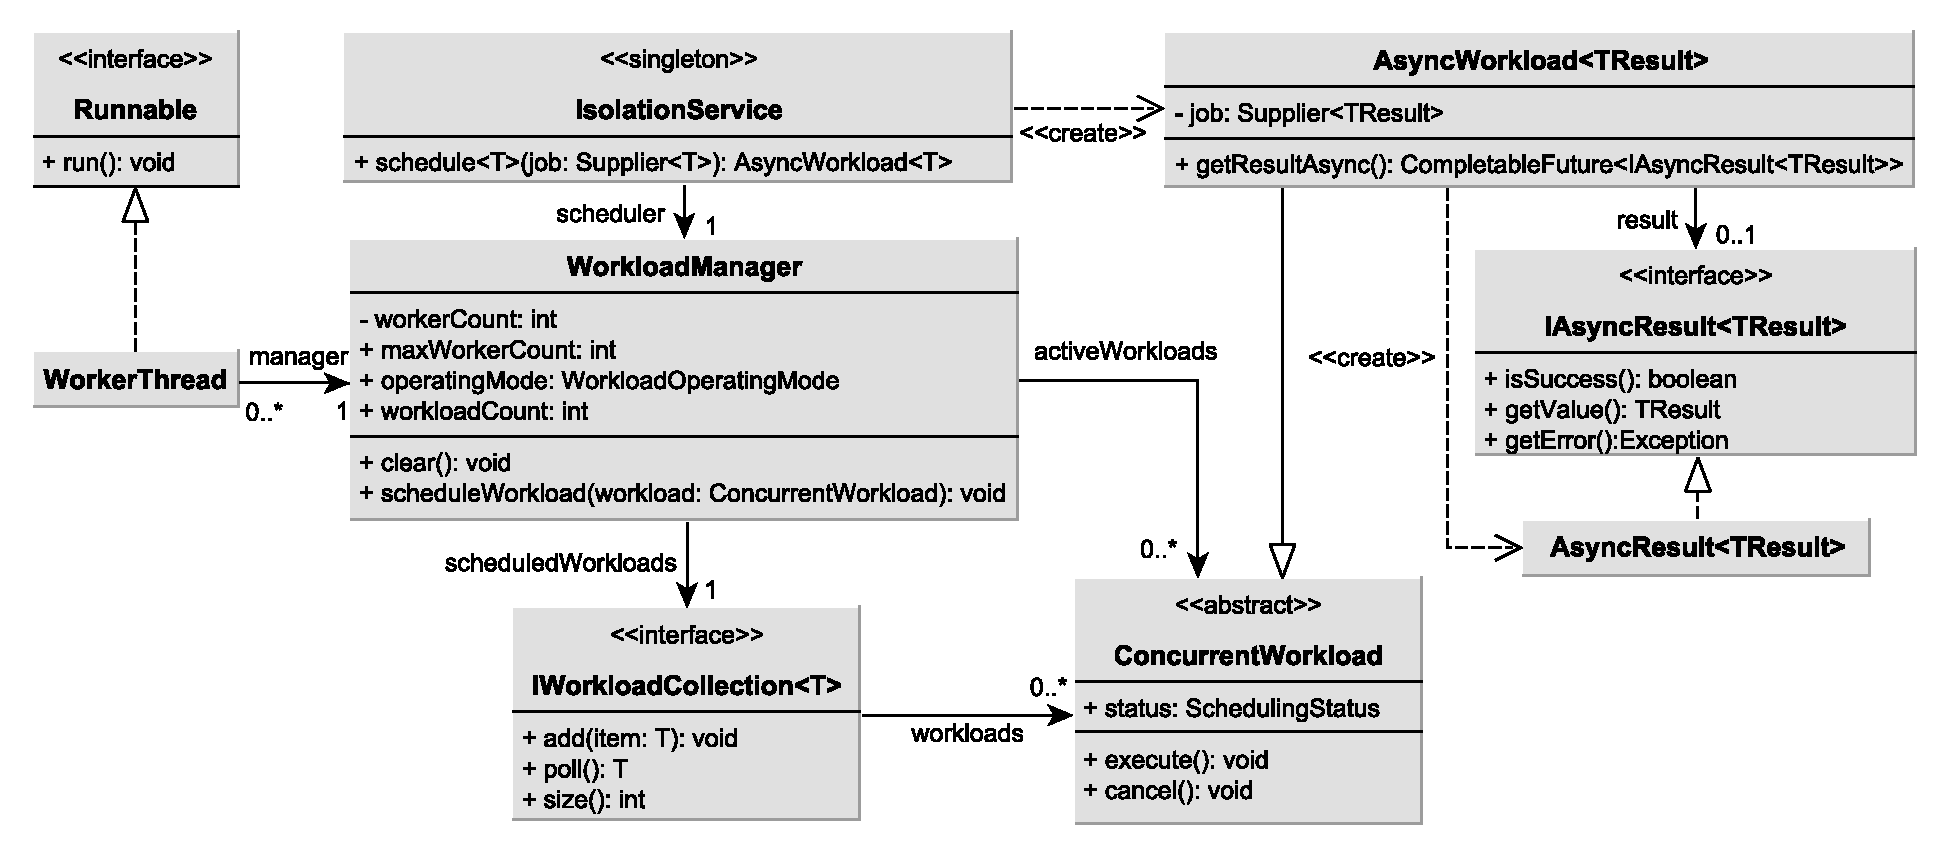
\includegraphics[width=\textwidth]{images/workload-management.pdf}
\caption{Simplified class diagram of the isolation service}
\label{fig:workload-overview}
\end{figure}

When scheduling an operation of type \inlinecode{Supplier<TResult>}, the \inlinecode{IsolationService} instantiates a new \inlinecode{AsyncWorkload<TResult>} object, which is then placed onto the dispatch queue and passed to the \inlinecode{WorkloadManager}. Subsequently, the isolation service returns the workload object to the caller, who can then obtain the \inlinecode{CompletableFuture<IAsyncResult<TResult>>} object from the workload instance and utilize it to block until the operation is completed and to retrieve the results.

Simultaneously, scheduling the workload induces the \inlinecode{WorkloadManager} to attempt to adjust the number of active workers. Initially, a synchronization lock is acquired to guarantee that the active worker count remains consistent while subsequent steps are performed. The \inlinecode{WorkloadManager} then checks if the maximum worker count has been reached; if not, the number of active workers is incremented by one, and a new worker thread is created. The caller releases the synchronization context and the new worker thread tries to dequeue workloads from the dispatch queue for execution. This process begins by acquiring another synchronization lock specific to the dispatch queue. Following this, another check is initiated to verify and adjust the worker counts, assuring that the new worker thread is still required and that the number of allowed threads was not altered since the last check.

If the upper boundary of threads has been violated, the worker thread terminates and another existing thread handles execution of the scheduled workload. Otherwise if the upper limit has not yet been reached and more workloads are available, an additional worker thread is created. In any case other than termination, the worker thread attempts to dequeue a workload from the dispatch queue. If the dispatch queue is empty, the thread decrements the active worker count by one, and terminates. Otherwise, the worker thread assesses whether the workload was canceled while waiting in the dispatch queue; if so, it retrieves the next workload from the queue. In any other ways, the workload is set to \inlinecode{SchedulingStatus.Executing}, forestalling attempts to cancel it, and the worker thread carries on with workload execution, invoking the provided lambda expression and storing the result by completing the corresponding \inlinecode{Future}  object in the \inlinecode{AsyncWorkload}. If an exception is raised in client code during execution, the Future is completed with the exception object. Finally, this process is repeated until the dispatch queue is empty, and the number of active workers is reduced to zero.

Once the \inlinecode{Future} object is completed, the calling \gls{a:api} controller thread unblocks, and a response is transmitted back to the client.

\pagebreak

\section{Client}\label{sec:cs-client}

This section presents the client application, which is the interface through which the user interacts with the system. The client application conforms to \cref{req:client-portability} (portability) by utilizing the most recent C\# 11/.NET 7 \gls{a:sdk}. C\# was chosen over Java, primarily due to a reduction of boilerplate code and greater portability, as the application can be published with a self-contained trimmed \gls{a:cclr}, eliminating the dependency on a separate .NET runtime installation. Additionally, the authors are more familiar with C\#, making it a natural choice.

\subsection{Introduction}

Despite being designed as a \glsfull{a:cli} without a \glsfull{a:gui}, the client strives to maintain an intuitive and user-friendly experience, enabling users to efficiently manage the cinema system on a day-to-day basis. Cinema employees utilize the application for creating, modifying, and deleting movies, cinema halls, seat rows, seats, and showtimes, while customers use it for booking and canceling tickets. Additionally, the client application supports administrative tasks, such as analyzing movie and showtime revenue. Consequently, the client application must differentiate between three use-case sets: \inlinecode{management}, \inlinecode{user}, and \inlinecode{administration} (abbreviated as \inlinecode{admin}).

To prioritize accessibility, commands are designed for intuitive and natural interaction. The first command layer corresponds to use-case groups, while the second layer denotes specific operations (\gls{a:crud}). Common aliases are provided for each command, allowing users to select their preferred syntax. Each command specifies a target for the operation, resulting in a three-part structure: the use-case group, specific operation, and target. For instance, \inlinecode{management create movie} and \inlinecode{user create booking} are valid commands. A \inlinecode{help} command facilitates \gls{a:cli} navigation, displaying available commands and options depending on the user's position within the command tree. For example, \inlinecode{management help} lists all available management commands, while \inlinecode{management create help} enumerates valid targets for the create command in the management context.

The subsequent sections delve into the components required for implementing these features. \Cref{sec:cs-cli} examines the \gls{a:cli} parser, \cref{sec:cs-api-access} discusses the infrastructure necessary for server access, and \cref{sec:cs-autocomplete} introduces the autocomplete layer.

\pagebreak

\subsection{Command line parsing}\label{sec:cs-cli}

A primary concern for the client involves developing an intuitive command line interface. To tackle this issue, the \inlinecode{System.CommandLine} framework is employed for parsing \gls{a:cli} commands and arguments. Consequently, a hierarchical command-argument structure is established to facilitate the interpretation of user input. The syntax tree depicted in \cref{fig:command-tree} illustrates the command structure available to the client. It is essential to note that the root node functions solely as a logical container for the main commands.
\begin{minipage}[t]{0.45\textwidth}
The child nodes of the root node comprise \inlinecode{management}, \inlinecode{user}, and \inlinecode{admin} commands, which align with the distinct use-case groups identified in \cref{sec:use-cases}. Management sub-commands are generalized into the \inlinecode{ManagementCommand} class, which defines common management target arguments, represented as enums, employed by the concrete \gls{a:crud} commands that extend the \inlinecode{ManagementCommand} class.

The user sub-tree is similarly divided into create, read, update, and delete commands. However, these sub-commands are not consolidated into a single class, as they may not share identical arguments. For example, customers can create ticket reservations and bookings, but only ticket reservations may be cancelled. An optional \inlinecode{--as-identity} option may be utilized to specify the user or customer identity for performing the designated action. If no identity is specified, the user% don't touch this lol
\end{minipage}
\hfill
\begin{minipage}[t]{0.6\textwidth}
\vspace{-.5cm}
\begin{figure}[H]
\renewcommand*\DTbaselineskip{10pt}
{\scriptsize
\dirtree{%
.1 root \type \syntaxcomplex{RootCommand}.
.2 management \extends \syntaxcomplex{Command}.
.3 \syntaxcomplex{ManagementCommand} \syntaxkeyword{<<abstract>>} \extends \syntaxcomplex{Command}.
.4 movies \type \syntaxprimitive{ManagementOperationTarget}.
.4 screenings \type \syntaxprimitive{ManagementOperationTarget}.
.4 halls \type \syntaxprimitive{ManagementOperationTarget}.
.4 rows \type \syntaxprimitive{ManagementOperationTarget}.
.4 seats \type \syntaxprimitive{ManagementOperationTarget}.
.3 create \extends \syntaxcomplex{ManagementCommand}.
.3 read \extends \syntaxcomplex{ManagementCommand}.
.3 update \extends \syntaxcomplex{ManagementCommand}.
.3 delete \extends \syntaxcomplex{ManagementCommand}.
.2 user \extends \syntaxcomplex{Command}.
.3 {-}-as-identity \type \syntaxcomplex{Option}.
.4 identity \type \syntaxprimitive{string}.
.3 create \extends \syntaxcomplex{Command}.
.4 user \type \syntaxprimitive{UserCreateCommandTarget}.
.4 booking \type \syntaxprimitive{UserCreateCommandTarget}.
.4 reservation \type \syntaxprimitive{UserCreateCommandTarget}.
.3 read \extends \syntaxcomplex{Command}.
.4 users \type \syntaxprimitive{UserReadCommandTarget}.
.4 bookings \type \syntaxprimitive{UserReadCommandTarget}.
.4 reservations \type \syntaxprimitive{UserReadCommandTarget}.
.3 update \extends \syntaxcomplex{Command}.
.4 reservation \type \syntaxprimitive{UserUpdateCommandTarget}.
.3 delete \extends \syntaxcomplex{Command}.
.4 user \type \syntaxprimitive{UserDeleteCommandTarget}.
.4 reservation \type \syntaxprimitive{UserDeleteCommandTarget}.
.3 book \syntaxkeyword{<<alias>>} \extends \syntaxcomplex{Command} $\implies$ create booking.
.3 reserve \syntaxkeyword{<<alias>>} \extends \syntaxcomplex{Command} $\implies$ create reservation.
.3 cancel \syntaxkeyword{<<alias>>} \extends \syntaxcomplex{Command} $\implies$ delete reservation.
.2 admin \extends \syntaxcomplex{Command}.
.3 show \extends \syntaxcomplex{Command}.
.4 revenue \type \syntaxprimitive{AdminReadCommandTarget}.
}
}
\renewcommand*\DTbaselineskip{20pt}
\caption{The client command syntax tree.}
\label{fig:command-tree}
\end{figure}
\end{minipage}
\vspace{-.25cm}

will be prompted to enter their respective email address in a subsequent step. Finally, a collection of alias commands are incorporated into the user command, which directly correspond to their respective \gls{a:crud} commands.

The admin sub-tree shares similarities with the user sub-tree but consists solely of the read command, employed to display the revenue of a specified movie or movie screening.

\pagebreak

\subsubsection{Class Design}

To implement \gls{a:cli} commands in a structured and maintainable fashion, the \inlinecode{System.CommandLine} framework is encapsulated within a class hierarchy, as illustrated in \vref{fig:command-classes}.

\begin{figure}[H]
    \centering
    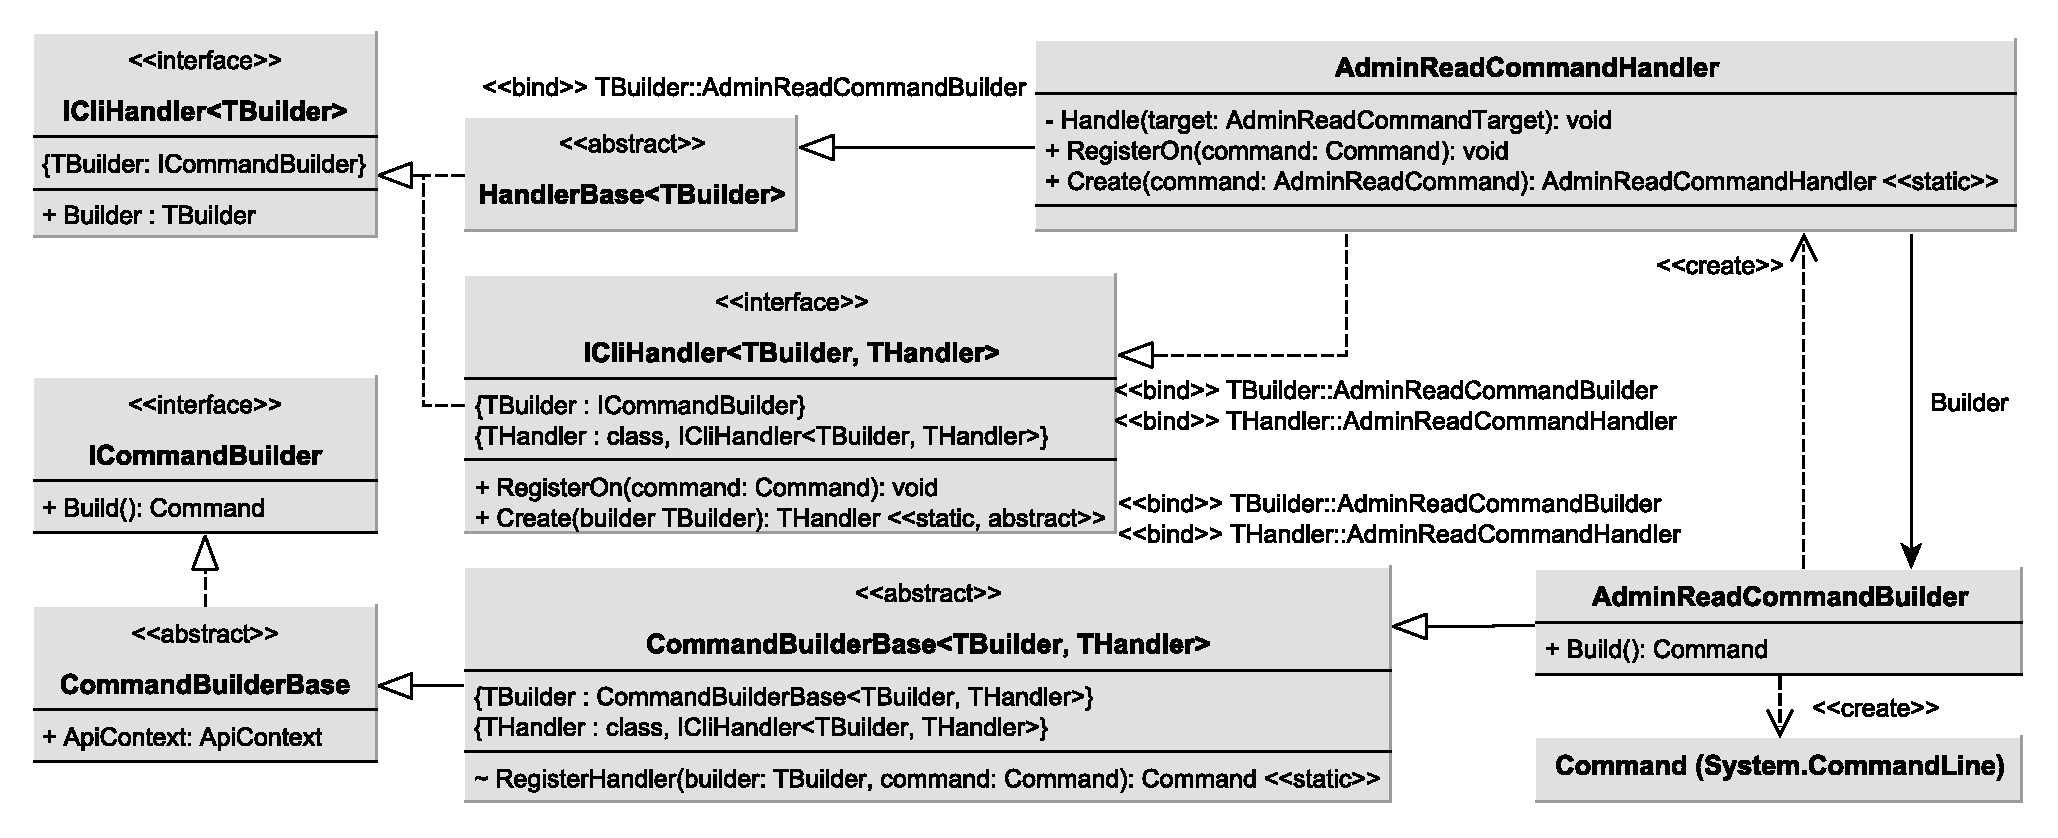
\includegraphics[width=\textwidth]{images/client-cli-command-parsing.pdf}
    \caption{Class hierarchy of the \gls{a:cli} command parsing framework.}
    \label{fig:command-classes}
\end{figure}

\Cref{fig:command-classes} displays the fundamental classes and interfaces of the command tree, along with an exemplary implementation of the \inlinecode{admin show} command.

The class hierarchy can be divided into command builders and command handler classes. Command builders serve to define and configure \inlinecode{System.CommandLine} command objects and their respective arguments. Command handler classes are responsible for configuring sub-commands on the \inlinecode{System.CommandLine} command objects within their corresponding \inlinecode{RegisterOn} methods and managing command execution through their \inlinecode{Handle} methods.

The configuration workflow generally adheres to the following steps:

\begin{enumerate}
    \item A command builder is instantiated and configured with the required arguments.
    \item The \inlinecode{builder.Build()} method is called to create and configure the \inlinecode{System.CommandLine} command object.
    \item The command object is added to the parent or root command object.
    \item The newly created command object is passed to the \inlinecode{RegisterHandler} method in the abstract \inlinecode{CommandBuilderBase} class, which subsequently generates the respective command handler using the static abstract \inlinecode{Create} factory method on the \inlinecode{THandler} type parameter.
    \item The \inlinecode{RegisterHandler} method calls the \inlinecode{RegisterOn} method on the command handler instance, which is accountable for registering sub-commands on the \inlinecode{System.CommandLine} command object. This is accomplished by instantiating one or more new command builders and passing them an instance of their corresponding parent, restarting from step 1.
\end{enumerate}

Consequently, each node in the syntax tree presented in \cref{fig:command-tree} is represented by an implementation of the \inlinecode{ICommandBuilder} interface, which in turn possesses a corresponding handler to recursively configure child command builder nodes. This arrangement offers a coherent and maintainable structure for the command tree, which can be effortlessly extended by incorporating new command builders and handlers for additional commands and their respective sub-commands.

A challenge presented by this command tree design involves the necessity to propagate global options, such as the \inlinecode{--as-identity} option in the user command sub-tree, from parent nodes to their child nodes. This is essential since the sole approach of obtaining the values of global options in the Handle methods of leaf nodes is via the original \inlinecode{System.CommandLine} option instance, configured by the parent command builder. As a result, any such options are stored within the respective command builder, which can then be injected into the corresponding command handler and passed down to subsequent layers of the command tree. To facilitate this process, C\# 11's support for static abstract interface members is employed. This enables the \inlinecode{Create} factory method to be defined and invoked using the associated generic type parameter \inlinecode{THandler}, mitigating the need for a separate factory object, or for explicit casts on the callee side if a generic factory were used \cite{ecma335cli-augments}. This design pattern is demonstrated in \cref{lst:command-builder-static-abstract-interface-members}.

\begin{listing}[H]
\begin{minted}[fontsize=\scriptsize,linenos,mathescape]{csharp}
public interface ICliHandler<TBuilder, THandler> : ICliHandler<TBuilder>
    where TBuilder : ICommandBuilder 
    where THandler : class, ICliHandler<TBuilder, THandler> 
{
    ...
    static abstract THandler Create(TBuilder builder); // static abstract factory method$\label{lst:ln:THandler-definition}$
}

public abstract class CommandBuilderBase<TBuilder, THandler> : CommandBuilderBase
    where TBuilder : CommandBuilderBase<TBuilder, THandler>
    where THandler : class, ICliHandler<TBuilder, THandler>
{
    ...
    // the generic RegisterHandler implementation
    protected static Command RegisterHandler(TBuilder builder, Command command)
    {
        // invocation of static method on the THandler type parameter which is known to 
        // implement the corresponding ICliHandler interface
        THandler handler = THandler.Create(builder); // use static interface method$\label{lst:ln:THandler-usage}$
        handler.RegisterOn(command);
        return command;
    }
}
\end{minted}
\vspace{-.25cm}
\caption{Utilization of a static abstract factory interface in the generic \inlinecode{RegisterHandler} implementation.}
\vspace{-.25cm}
\label{lst:command-builder-static-abstract-interface-members}
\end{listing}

\Vref{lst:command-builder-static-abstract-interface-members} presents the definition of the static abstract factory method in \inlinecode{ICliHandler} in \lref{lst:ln:THandler-definition} and its usage in the generic implementation of the \inlinecode{RegisterHandler} method in \lref{lst:ln:THandler-usage}. Generic constraints on the type parameters of \inlinecode{CommandBuilderBase} and \inlinecode{ICliHandler} ensure the appropriate command handler is created and registered for the corresponding command builder, eliminating the need for explicit casts or type checking.

\subsection{API Access}\label{sec:cs-api-access}

Upon command execution, the corresponding command handler class assumes responsibility for managing the command's execution.

Since the majority of leaf nodes in the command tree correspond to enums, the respective enum value is passed to the command handler, which subsequently switches on its value and invokes the appropriate \inlinecode{RemoteOperation} delegate. The \inlinecode{RemoteOperation} delegate refers to a method in the associated \inlinecode{Operation} class, which is specific to the handler and is accountable for performing one or more \gls{a:api} calls relevant to the requested operation. This approach enables command handler classes to remain independent of the actual \gls{a:api} calls, concentrating solely on managing the command's execution and promoting a cleaner separation of concerns. The hierarchy of user operation classes depicted in \cref{fig:client-operations} serves as a representative example for other operation class hierarchies.

\begin{figure}[H]
    \centering
    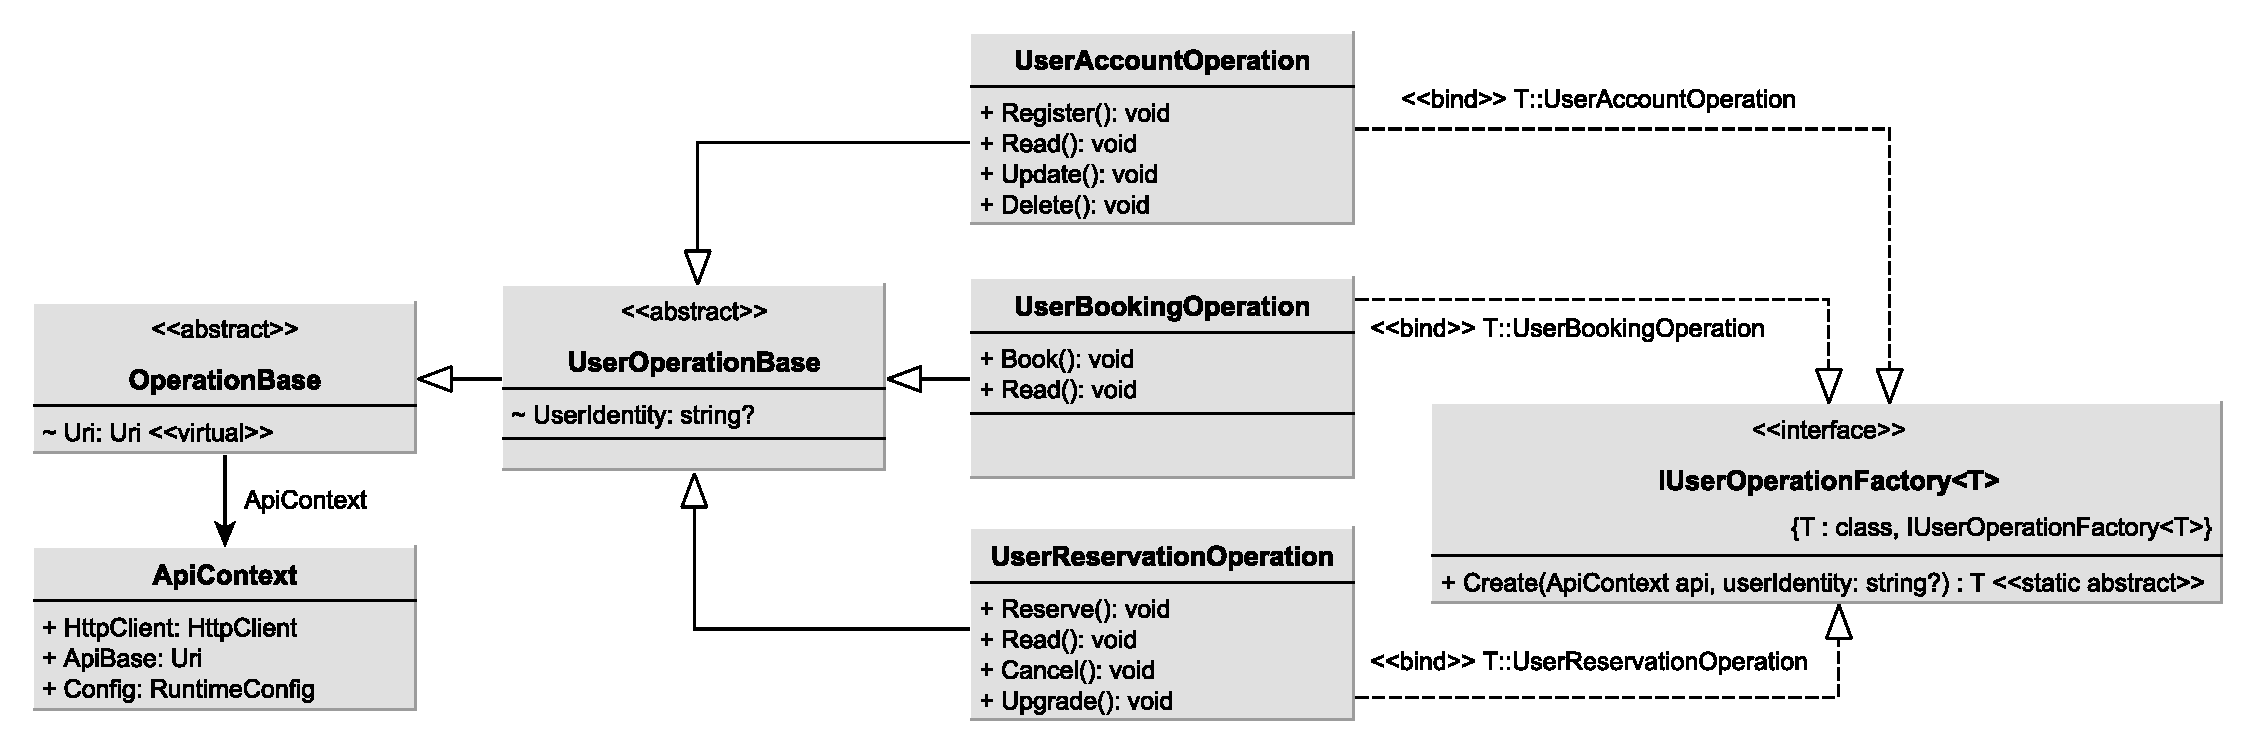
\includegraphics[width=\textwidth]{images/client-operations}
    \caption{User operation class hierarchy.}
    \label{fig:client-operations}
\end{figure}


As illustrated in \cref{fig:client-operations} the \inlinecode{OperationBase} class maintains a reference to an \inlinecode{ApiContext} object, responsible for storing the \inlinecode{HttpClient} instance utilized for all \gls{a:api} calls, as well as the server's base \gls{a:uri}. This ensures that each operation uses the same \inlinecode{HttpClient} instance and thus, the same connection pool, which is crucial for performance considerations. Upon creation of an operation object, it receives a reference to the \inlinecode{ApiContext} object, which is subsequently stored in the corresponding property. Additionally, every operation class has a \inlinecode{Uri} property, initialized in the constructor, that represents the relative path from the server's base \gls{a:uri} to the corresponding \gls{a:api} controller that manages the requested operation.

When an operation is executed by the command handler, the \inlinecode{Uri} property is queried to construct the absolute \gls{a:uri} of the desired \gls{a:api} controller. Depending on the operation, one or more \gls{a:api} calls are performed to aggregate data necessary for user interaction, displaying results, or executing the requested operation. Once the operation is complete, the client application terminates.

\subsection{Autocomplete Wrapper}\label{sec:cs-autocomplete}

Given that the client itself is a command line application with the capacity to execute only one command at a time, an additional wrapper application has been implemented to provide dynamic autocompletion and syntax highlighting based on the command syntax tree defined in the client. As this wrapper is also developed in C\#, it can import the client executable as a dependency, enabling the generation of a syntax tree of autocompletion node data based on the command tree defined in the client. This facilitates seamless integration of the client application into the shell environment. The wrapper application also maintains an additional command history stack, allowing for quick navigation through previously executed commands. The architecture of the wrapper application is depicted in \cref{fig:client-wrapper}.

\begin{figure}[H]
    \centering
    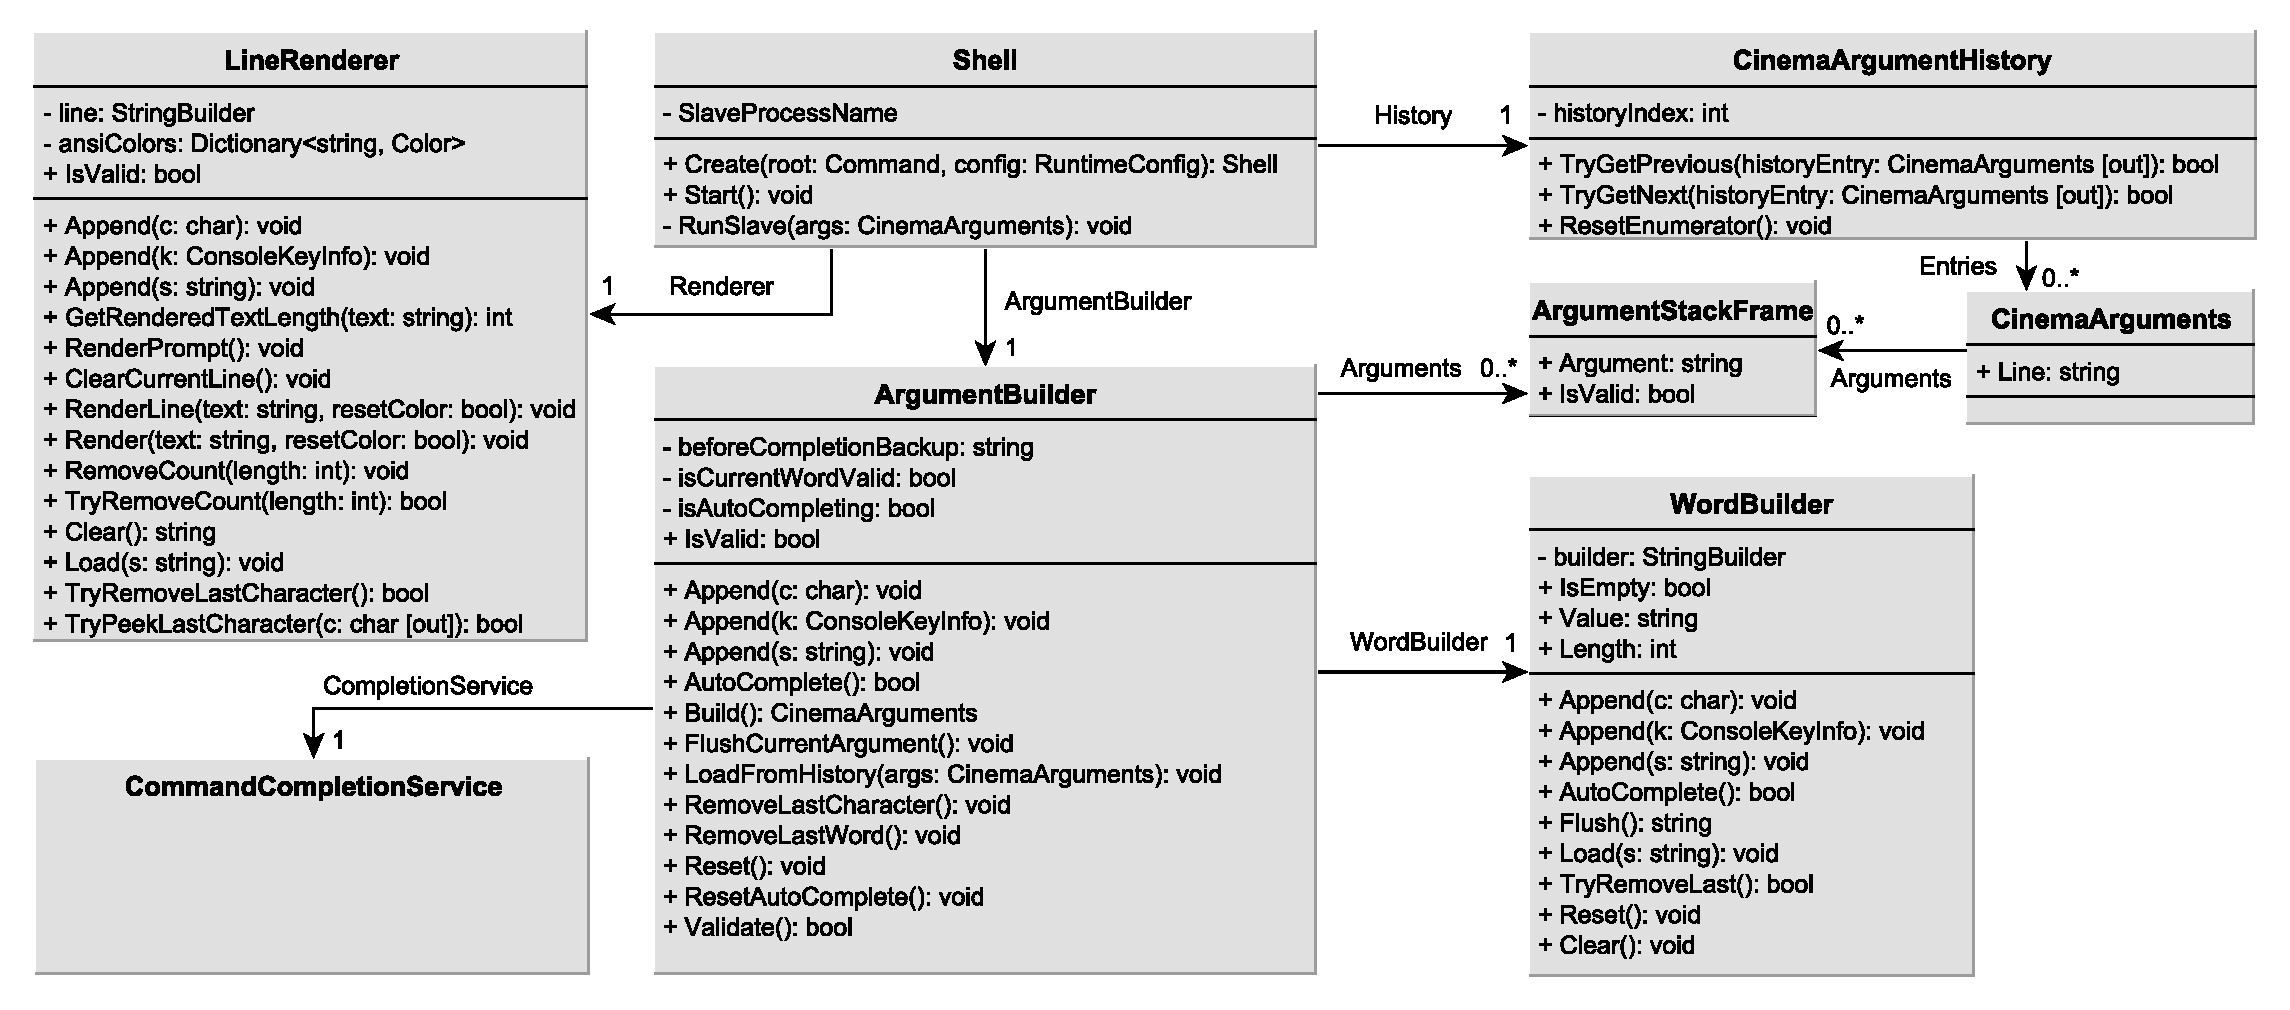
\includegraphics[width=\textwidth]{images/client-wrapper}
    \caption{Architecture of the client wrapper application.}
    \label{fig:client-wrapper}
\end{figure}

As shown in Figure \ref{fig:client-wrapper}, the core class of the wrapper is the \inlinecode{Shell} class, which is responsible for monitoring key presses, managing dependent classes, and slaving the client application to the current command line.

When the \inlinecode{Shell::Start()} method is invoked, a prompt is rendered to the screen using the \inlinecode{LineRenderer} class, which also offers support for parsing \gls{a:ansi} color codes. As soon as a key press event is raised, the following parsing algorithm is executed:

\begin{enumerate}
    \item The key information is read, and depending on the character, one of these actions is taken:
    \begin {enumerate}
        \item For alphanumeric \gls{a:ascii} characters or symbols, the character is appended to the \inlinecode{ArgumentBuilder} and \inlinecode{LineRenderer}. The \inlinecode{ArgumentBuilder} updates its internal \inlinecode{WordBuilder} instance accordingly.
        \item For arrow keys (up or down), the previous or next command from the command history is retrieved using the \inlinecode{CinemaArgumentsHistory} class. The \inlinecode{ArgumentBuilder} and \inlinecode{LineRenderer} are updated, the prompt is redrawn, and the key parsing process \textbf{concludes} and is ready to handle the next key press.
        \item For a backspace key, the last character or word (depending on whether the control key is also pressed) is removed from the \inlinecode{ArgumentBuilder} and \inlinecode{LineRenderer}. The \inlinecode{ArgumentBuilder} updates its internal \inlinecode{WordBuilder} instance accordingly.
        \item For a space or enter key, the \inlinecode{ArgumentBuilder} flushes it's current word, validates the new argument against the syntax tree by invoking the \inlinecode{CommandCompletionService}, and pushes the argument onto the argument stack.
        \begin{enumerate}
            \item If the enter key is pressed, the renderer completes the current line, the \inlinecode{ArgumentBuilder} is flushed, and a new line is rendered. The client application is then spawned as a slave process, forwarding input, output, and error streams to the master. When the client process exits, the key parsing \textbf{concludes} and is ready to handle the next key press.
            \item Otherwise, if the key is a space, the space character is added to the renderer.
        \end{enumerate}
        \item Any other keys are ignored for now.
    \end{enumerate}
    \item The \inlinecode{ArgumentBuilder} validates its current argument stack and partial argument against the syntax tree.
    \begin{enumerate}
        \item If the argument is valid, it is passed to the \inlinecode{CommandCompletionService}, and the autocomplete cache is updated accordingly. The \inlinecode{CommandCompletionService} returns a list of possible completions for the current argument.
        \item Otherwise, the renderer is updated to re-render the current line in red for the next call to \inlinecode{RenderPrompt()}.
    \end{enumerate}
    \item One of the following actions is taken:
    \begin{enumerate}
        \item If the key is a tab key, the current partial input is backed up, and one of these actions is taken:
        \begin{enumerate}
            \item If the autocomplete cache is empty, the cache is updated by invoking the \inlinecode{CommandCompletionService} with the current argument.
            \item Otherwise, the autocomplete cache is queried for possible completions for the current argument.
            \begin{enumerate}
                \item If the previous key was also a tab key, the next completion in the autocomplete cache is returned.
                \item Otherwise, the first completion in the autocomplete cache is returned.
                \item If the autocomplete cache is empty or no next completion exists, the backup is restored.
            \end{enumerate}
            \item The \inlinecode{ArgumentBuilder} and \inlinecode{LineRenderer} are updated with the new completion.
        \end{enumerate}
        \item Otherwise, the autocomplete cache is reset.
    \end{enumerate}
    \item The current line is re-rendered.
    \item The key parsing concludes and is ready to handle the next key press.
\end{enumerate}

Overall, the shell wrapper aims to provide seamless integration of the client application into the shell environment, enabling a more intuitive user experience.

\chapter{Implementation}
\label{ch:impl}

All proposed concepts have been realized in a \gls{g:cms} prototype. This chapter outlines crucial design choices and implementation specifics, including necessary modifications to the architecture and lessons learned throughout the process. Ultimately, the prototype is evaluated against the requirements delineated in \cref{sec:requirements}.

\section{HTTP Response Model Mapping}\label{sec:impl-lombok}

One modification made to the original architecture presented in \vref{fig:architecture} involves incorporating the Project Lombok code generation library to assist with the implementation of the \gls{a:json} \gls{a:rrm}. Adhering to the core principles of \gls{a:mdd}, Lombok is a Java library that employs a higher-level representation of a Java class to automatically generate implementation details, such as getter and setter methods for fields, at compile time. \Cref{fig:architecture-with-lombok} reflects the resulting changes to the project architecture.

\begin{figure}[H]
\centering
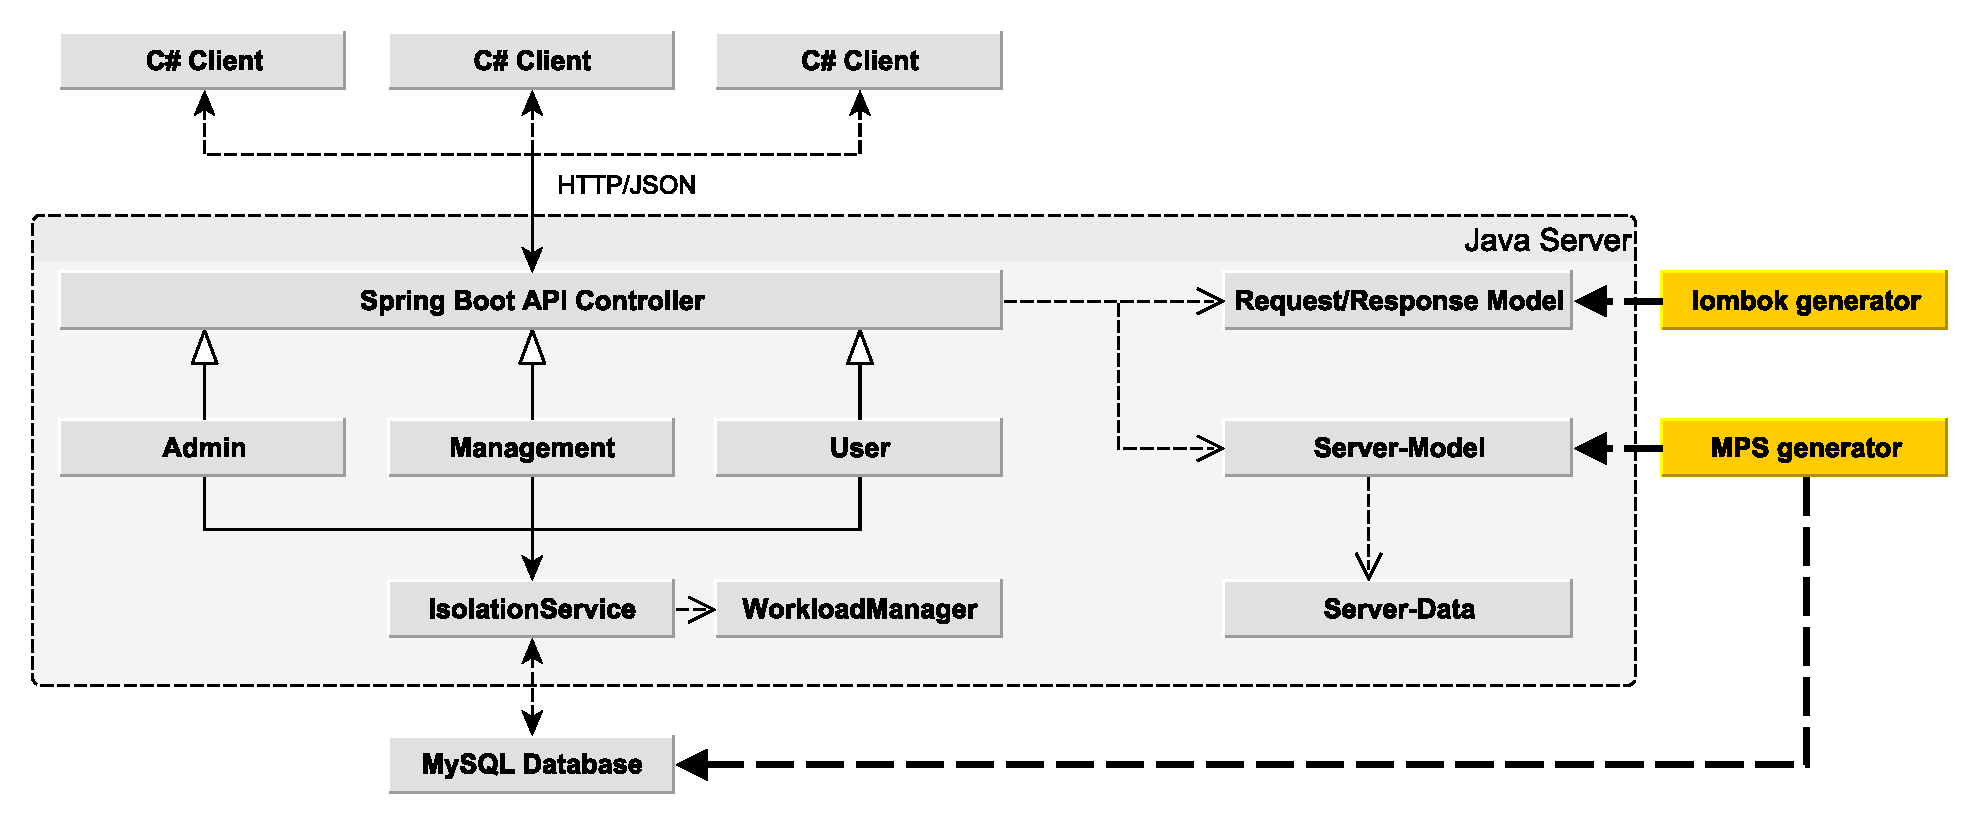
\includegraphics[width=\textwidth]{images/big-picture}
\caption{The final project architecture following the integration of Lombok.}
\label{fig:architecture-with-lombok}
\end{figure}

In the prototype, the \inlinecode{@Data} annotation was utilized to generate getter and setter methods for each field. This annotation was applied to all \gls{a:rrm} classes in the \gls{g:cms} prototype, reducing the amount of boilerplate code that needed to be written. This enhancement in code maintainability was accomplished with minimal effort and proved to be a significant time-saver, allowing the development team to concentrate more on implementing the actual functionality. The example provided in \vref{lst:lombok-example} demonstrates the advantages of using Lombok.

\begin{figure}[H]
\begin{minipage}[t]{0.5\textwidth}
\begin{minted}[fontsize=\scriptsize,linenos]{java}
public class UserUpgradeReservationRequest {
    private Integer reservationId;
    private String email;
    public Integer getReservationId() {
        return this.reservationId;
    }
    public void setReservationId(Integer value) {
        this.reservationId = value;
    }
    public String getEmail() {
        return this.email;
    }
    public void setEmail(String value) {
        this.email = value;
    }
}
...
String email = request.getEmail(); // works
\end{minted}
\end{minipage}
\hfill
\begin{minipage}[t]{0.5\textwidth}
\begin{minted}[fontsize=\scriptsize,linenos]{java}
@Data
public class UserUpgradeReservationRequest {
    Integer reservationId;
    String email;
}
...
String email = request.getEmail(); // works
\end{minted}
\end{minipage}
\captionof{listing}{The same class before and after applying the \inlinecode{Data} annotation}
\label{lst:lombok-example}
\end{figure}

\Cref{lst:lombok-example} demonstrates the \inlinecode{UserUpgradeReservationRequest} class before and after applying the \inlinecode{Data} annotation. The \inlinecode{Data} annotation automatically generates getter and setter methods for each field, which are then utilized in the same manner as in the original, manually written class. The code in the \inlinecode{UserUpgradeReservationRequest} class is reduced from 16 lines to 5 lines, corresponding to a 69\% reduction in boilerplate code. This decrease in boilerplate code leads to a substantial improvement in the project's maintainability, as less code needs to be written and managed.

\section{Reflective Object Mapping}\label{sec:impl-reflective-object-mapping}

An optimization applied to the \gls{a:rrm} implementation involved the addition of the \inlinecode{ObjectX} (Object Extensions) class. \inlinecode{ObjectX} offers a suite of reflection-based methods for populating a response object based on a given \gls{a:mps}-generated data model instance. Utilizing reflection, the \inlinecode{ObjectX} class identifies shared properties with matching names and data types between the two classes. Subsequently, a new instance of the response class is created, and values are transferred from the data model instance to the response class instance. \Cref{lst:reflective-object-mapping-example} demonstrates this process.

\begin{listing}[H]
\begin{minted}[fontsize=\scriptsize,linenos,mathescape]{java}
@GetMapping("/list")
public ResponseEntity<GetMoviesResponse> listMovies() 
{
    return isolated(() -> 
    {
        GetMoviesResponse response = new GetMoviesResponse();
        response.setMovies(ObjectX.createFromMany(               // ObjectX usage$\label{lst:objectx:ln:usage}$
            CinemaService.getInstance().getMovieCache().values(), 
            GetMoviesResponseEntry.class));
        response.setSuccess(true);
        return new ResponseEntity<GetMoviesResponse>(response, HttpStatus.OK);
    });
}
\end{minted}
\vspace{-.5cm}
\caption{Example of a controller method using the \inlinecode{ObjectX} class to efficiently transform a data model instance to a response model instance.}
\label{lst:reflective-object-mapping-example}
\end{listing}

\Vref{lst:reflective-object-mapping-example} presents an example of the \inlinecode{MovieController} class utilizing the \inlinecode{ObjectX} class in \lref{lst:objectx:ln:usage} for the efficient conversion of a collection of \inlinecode{Movie} instances into a set of \inlinecode{GetMoviesResponseEntry} response model instances.

In combination with the lombok-annotated response model classes, the overhead associated with modeling \gls{a:json} \glspl{a:rrm} is minimized, leading to a substantial enhancement in development speed.

\section{Challenges and limitations}\label{sec:impl-challenges}

During development of the prototype, a number of challenges were encountered, some of which are discussed in this section.

\subsection{Inserting Default Values for \headercode{PriceCategories}}

As per the data model defined in \cref{sec:cs-data-model}, the \inlinecode{PriceCategory} class owns a \inlinecode{price} attribute. This attribute, intended to be of type \inlinecode{Rational}, corresponds to the ticket price for a given \inlinecode{PriceCategory}. As the default values are not part of the data model, the \inlinecode{price} attribute must be initialized with a value before being accessed by the application. The goal was to eagerly initialize the \inlinecode{price} upon the server startup. To accomplish this, the guard clause illustrated in \cref{lst:price-category-initialization} was added to the main method of the \gls{g:cms}:

\begin{listing}[H]
\begin{minted}[fontsize=\scriptsize]{java}
@SpringBootApplication
public class Program 
{
    public static void main(String[] args) 
    {
        if (!PriceCategoryStalls.getInstance().getPrice().isPresent())
        {
            PriceCategoryStalls.getInstance().setPrice(new Rational(10));
            PriceCategoryBox.getInstance().setPrice(new Rational(12));
            PriceCategoryServiceBox.getInstance().setPrice(new Rational(16));
        }
        SpringApplication.run(Program.class, args);
    }
}
\end{minted}
\caption{Guard clause for initializing default values of price categories.}
\label{lst:price-category-initialization}
\end{listing}

\Cref{lst:price-category-initialization} demonstrates the initialization of \inlinecode{PriceCategory} instances with default values if they are unset. However, this attempt to initialize default values did not yield the expected results. Although the \inlinecode{PriceCategoryBox} and \inlinecode{PriceCategoryServiceBox} singleton instances were initialized correctly, the \inlinecode{PriceCategoryStalls} instance was not. Further testing revealed that the first price category to be initialized would always fail, while subsequent attempts to initialize the corresponding price category would also prove unsuccessful. Other price categories could be initialized correctly, but the first price category would consistently fail. Due to time constraints, this issue could not be investigated further during development of the prototype. Consequently, the price attribute was temporarily removed from the data model, and offline price calculations were implemented based on the class type of a given \inlinecode{PriceCategory} instance.

Future work should thoroughly investigate this issue to determine the root cause and establish whether the bug originates in \gls{g:cms} or the generated data access layer.

\subsection{Inconsistent Database States and Missing Transactions}

The absence of database transactions generated by \gls{a:mps} significantly hindered the prototype development. Although concurrency issues were addressed using the isolation service described in \cref{sec:cs-isolation}, the lack of transactions prevented the data access layer from rolling back database changes in the event of an error. This issue manifested in the server application crashing randomly during subsequent data access operations, leading to considerable frustration during development. Consequently, until the error sources could be identified and resolved, the database was dropped and the \gls{a:mps} generator re-run each time the server was restarted during development. This practice resulted in a substantial increase in development time, as test data had to be re-entered every time the server was restarted.

Future work should prioritize extending the \gls{a:mps} generator to create accurate transactional data access code before deploying the prototype in a production environment.

\pagebreak

\section{Requirement validation}
\label{sec:ProjectReview}

The proposed conceptual solution was implemented in a pre-production prototype of the \gls{g:cms} and tested against the requirements identified in \cref{sec:requirements}. The results of the requirement validation are presented in \vref{tab:requirement-validation-results}.

\renewcommand{\arraystretch}{1.25}
\begin{table}[H]
    \centering
    \caption{Validation of requirements.}
    \label{tab:requirement-validation-results}
    \begin{tabular}{l|p{0.75\textwidth}}
        \toprule
        Requirement & Validation \\
        \midrule
        \ref{req:use-cases} &  \lorizzleshortnospace \\ \hline
        \ref{req:model-requirements} &  \lorizzleshortnospace \\
        \bottomrule
    \end{tabular}
\end{table}
\renewcommand{\arraystretch}{1}
\chapter{Conclusion}
\label{ch:conclusion}

This work presented a case study that highlighted easily exploitable attack vectors that most anti-virus engines failed to detect. It was determined that threat actors could utilize these adversarial approaches to extract confidential information from the virtual memory of a running process. Moreover, the limitations and shortcomings of existing methods for protecting sensitive data in memory in .NET (primarily a lack of portability) were identified and translated into requirements for a new solution called XXX. \todo{copy-pasted from Ubi :P}

\todo{Jana´s Vorschlag}
In this work, a network-based cinema management system was successfully developed that implements all the requirements presented previously. The requirements were first identified with the help of a use case, which was then translated into a class diagram. The class model could be used for automated code generation with MPS, as it contains all the essential requirements. With a few changes, the generated code could contribute to the successful implementation of the management system with regulated network communication between client and server. 
Overall, it can be said that the generated code was difficult to integrate into the implementation because it does not take into account the undesired effects of network communication and therefore does not prevent them. Therefore, some changes had to be made here.

\section{Evaluation}
Overall, it can be stated that the cinema management system fulfills all requirements from chapter \ref{ch:problem-analysis}. These could be presented in a live demonstration of a use case using a console output. Here, the owner was able to successfully create cinema halls, movies and movie shows. Customers could first create a user account and then choose between different movies. These could either be booked or reserved. In doing so, the customer has to choose the price category, the row of seats and the seat. Reservations could be canceled and bookings cannot be canceled, in this case the customer gets a meaningful error message. The customer can convert a reservation into a booking. Furthermore, a competitive access to a seat of the same row of the same movie could be shown. It could be demonstrated that only one customer could book the seat and the other received an error message that this seat was already occupied. All in all, this application worked completely error-free during the live demonstration and the implementation of the task can be considered a success.


\section{Future Development Prospects}
\label{sec:outlook}


\todo{Ctrl+F for "future" or "further"}
\todo{Further research is required... to figure out how to actually insert PriceCategory values into the DB on application startup (the thing that refused to work for us lol)}

\lorizzleshort

\lorizzleshort

\section{Final thoughts}

\lorizzle


%%%----------------------------------------------------------
%                        Schlussteil
%%%----------------------------------------------------------

\lists
\listoflistings
\addcontentsline{toc}{chapter}{List of Listings}

\printnoidxglossary[type=\acronymtype, sort=word]
\printnoidxglossary[sort=word]

\MakeBibliography %Quellenverzeichnis

\appendixpage

%\appendixchapter{Extended theoretical foundation}
\label{apx:ch:extended-foundation}

\appendixchapter{Additional Requirements}
\label{apx:ch:extended-analysis}

\renewcommand{\arraystretch}{1.25}
\begin{table}[H]
    \centering
    \caption{Summary of model requirements for \gls{g:cms}.}
    \label{apx:tab:model-requirements}
    \begin{tabular}{l|p{0.75\textwidth}}
        \toprule
        Model Requirement & Description \\ \midrule
        \modelrequirementdefshort\label{req-mdl:cinema} & we need a cinema \\ \hline
        \modelrequirementdefshort\label{req-mdl:other} & some other stuff. \\ \hline
        \modelrequirementdefshort\label{req-mdl:foo} & \lorizzleshortnospace \\
        \bottomrule
    \end{tabular}
\end{table}
\renewcommand{\arraystretch}{1}

Referencing \cref{req-mdl:other} works. \Cref{req-mdl:cinema} is also defined? yup :)
%\appendixchapter{Extended implementation}

This appendix chapter provides additional implementation details for the features implemented in this work.

%\appendixchapter{Performance benchmarks}
\label{apx:chap:perf-benchmarks}

This appendix chapter presents the performance benchmarks conducted for this work.

%\appendixchapter{Full implementations}

This appendix chapter provides the complete implementations of some of the features presented in earlier sections of this work.


\end{document}